\documentclass[12pt, a4paper]{article}

% Paquetes esenciales
\usepackage[utf8]{inputenc}
\usepackage[spanish]{babel}
\usepackage{graphicx}
\graphicspath{{img/}{./}}
\usepackage{geometry}
\geometry{top=2.5cm, bottom=2.5cm, left=3cm, right=3cm}
\usepackage{hyperref}
\usepackage{float}
\usepackage{titlesec}
\usepackage{fancyhdr}

% Configuración de encabezado y pie de página
\pagestyle{fancy}
\fancyhf{}
\rhead{Proyecto Entregable 1}
\lhead{Ingeniería de Datos y Big Data}
\cfoot{\thepage}

\begin{document}

% Portada
\begin{titlepage}
    \centering
    \vspace*{2cm}
    
    {\Large \textbf{Universidad Católica del Norte}}\\[0.5cm]
    {\large Escuela de Ingeniería}\\[0.2cm]
    {\large Sede Coquimbo}\\[0.2cm]
    {\large Ingeniería en Tecnologías de Información}\\[3cm]
    
    {\Huge \textbf{Proyecto de Reportabilidad (ETL)}}\\[1cm]
    {\Large \textbf{Entregable 1: Arquitectura, Diseño de Reportes y Base de Datos OLTP}}\\[3cm]
    
    \begin{flushright}
    \large
    \textbf{Autores:}\\
    Martín Castillo Torrejón\\
    Daniel Durán García \\[1cm]
    
    \textbf{Asignatura:}\\
    Ingeniería de Datos y Big Data\\[1cm]
    
    \textbf{Fecha de Entrega:}\\
    Lunes 14 de Septiembre de 2026
    \end{flushright}
    
    \vfill
\end{titlepage}

\tableofcontents
\newpage

\section{Introducción}
El presente documento detalla la primera fase del desarrollo de la plataforma de reportabilidad para Adventure Works Cycles. En esta etapa inicial, se aborda el diseño de la arquitectura de la solución orientada a Business Intelligence, el diseño conceptual de los reportes para las perspectivas estratégicas de la empresa, y la implementación de la fuente de datos transaccional (OLTP).

%-----------------------------------------------------------------------

\section{Diseño de la Arquitectura de la Solución}
En esta sección se presenta el flujo de los datos desde su origen hasta su visualización, omitiendo la capa de cubos de datos (Semántica BI) según los requerimientos de la asignatura.

\begin{figure}[H]
    \centering
    
\includegraphics[width=0.88\textwidth]{arquitectura.png}
    \caption{Arquitectura de la solución para Adventure Works.}
    \label{fig:arquitectura}
\end{figure}

El flujo consta de las siguientes capas:
\begin{itemize}
    \item \textbf{Fuente de Datos (OLTP):} Base de datos transaccional alojada en SQL Server.
    \item \textbf{ETL:} Proceso de Extracción, Transformación y Carga.
    \item \textbf{Repositorio de Datos (Data Warehouse):} Almacén estructurado en modelo dimensional.
    \item \textbf{Visualización y Dashboards:} Capa final en Power BI para el consumo de los usuarios ejecutivos.
\end{itemize}
Además, se consideran las capas transversales correspondientes a Seguridad, Gobierno de Datos, Monitoreo y Backup.

%-----------------------------------------------------------------------

\clearpage
\section{Diseño de los Reportes Solicitados}
A continuación, se presentan los \textit{mockups} (bosquejos) de los tableros de control solicitados, distribuidos en tres perspectivas clave del negocio. Cada perspectiva contiene al menos cinco indicadores o gráficos estratégicos.

\subsection{Perspectiva de Clientes}
Se proponen los siguientes 5 reportes:
\begin{enumerate}
    \item \textbf{C1. Perfil de clientes:} Conocer la composición de la cartera de clientes. Medirá clientes totales, clientes individuales, clientes empresa/tienda y porcentaje de cada tipo.
    \nopagebreak
    \begin{figure}[H]
        \centering
        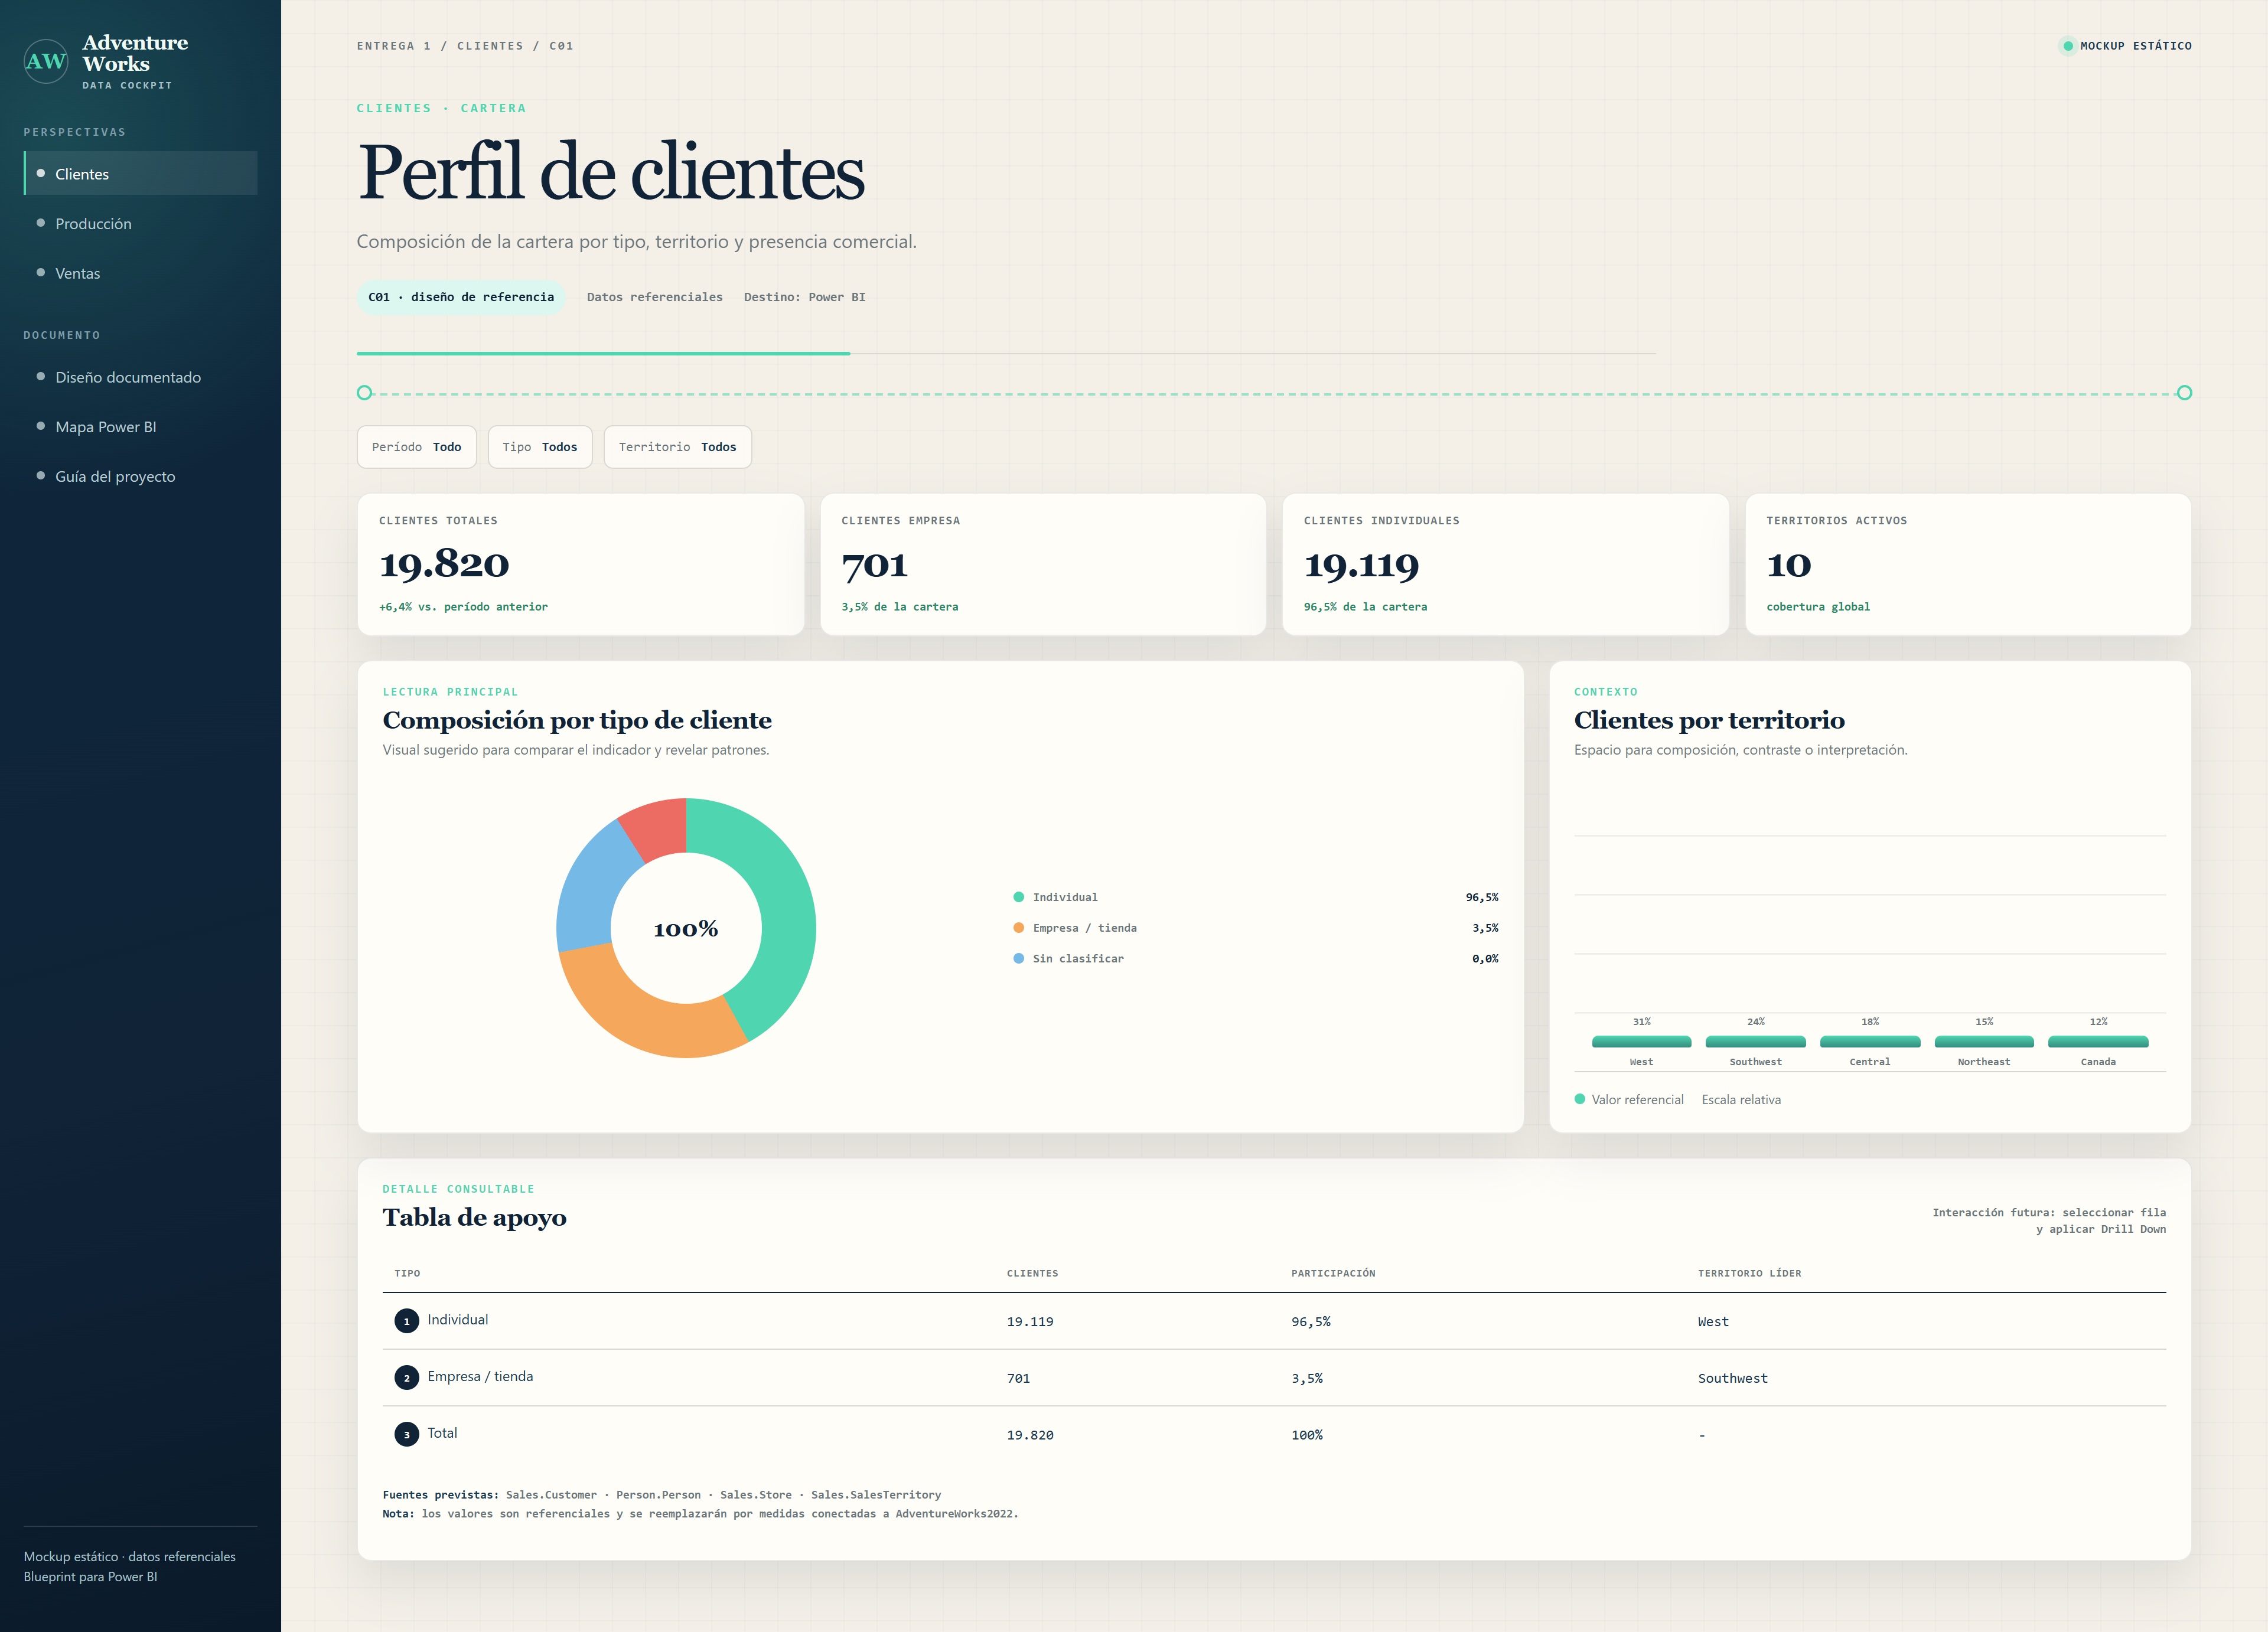
\includegraphics[width=0.82\textwidth]{mockup_clientes_01-perfil-clientes.png}
        \caption{Reporte C1: Perfil de clientes.}
    \end{figure}
    
    \clearpage
    \item \textbf{C2. Ventas por cliente:} Identificar los clientes que generan más ingresos. Medirá ventas totales, cantidad de órdenes, ticket promedio y participación del Top 10.
    \nopagebreak
    \begin{figure}[H]
        \centering
        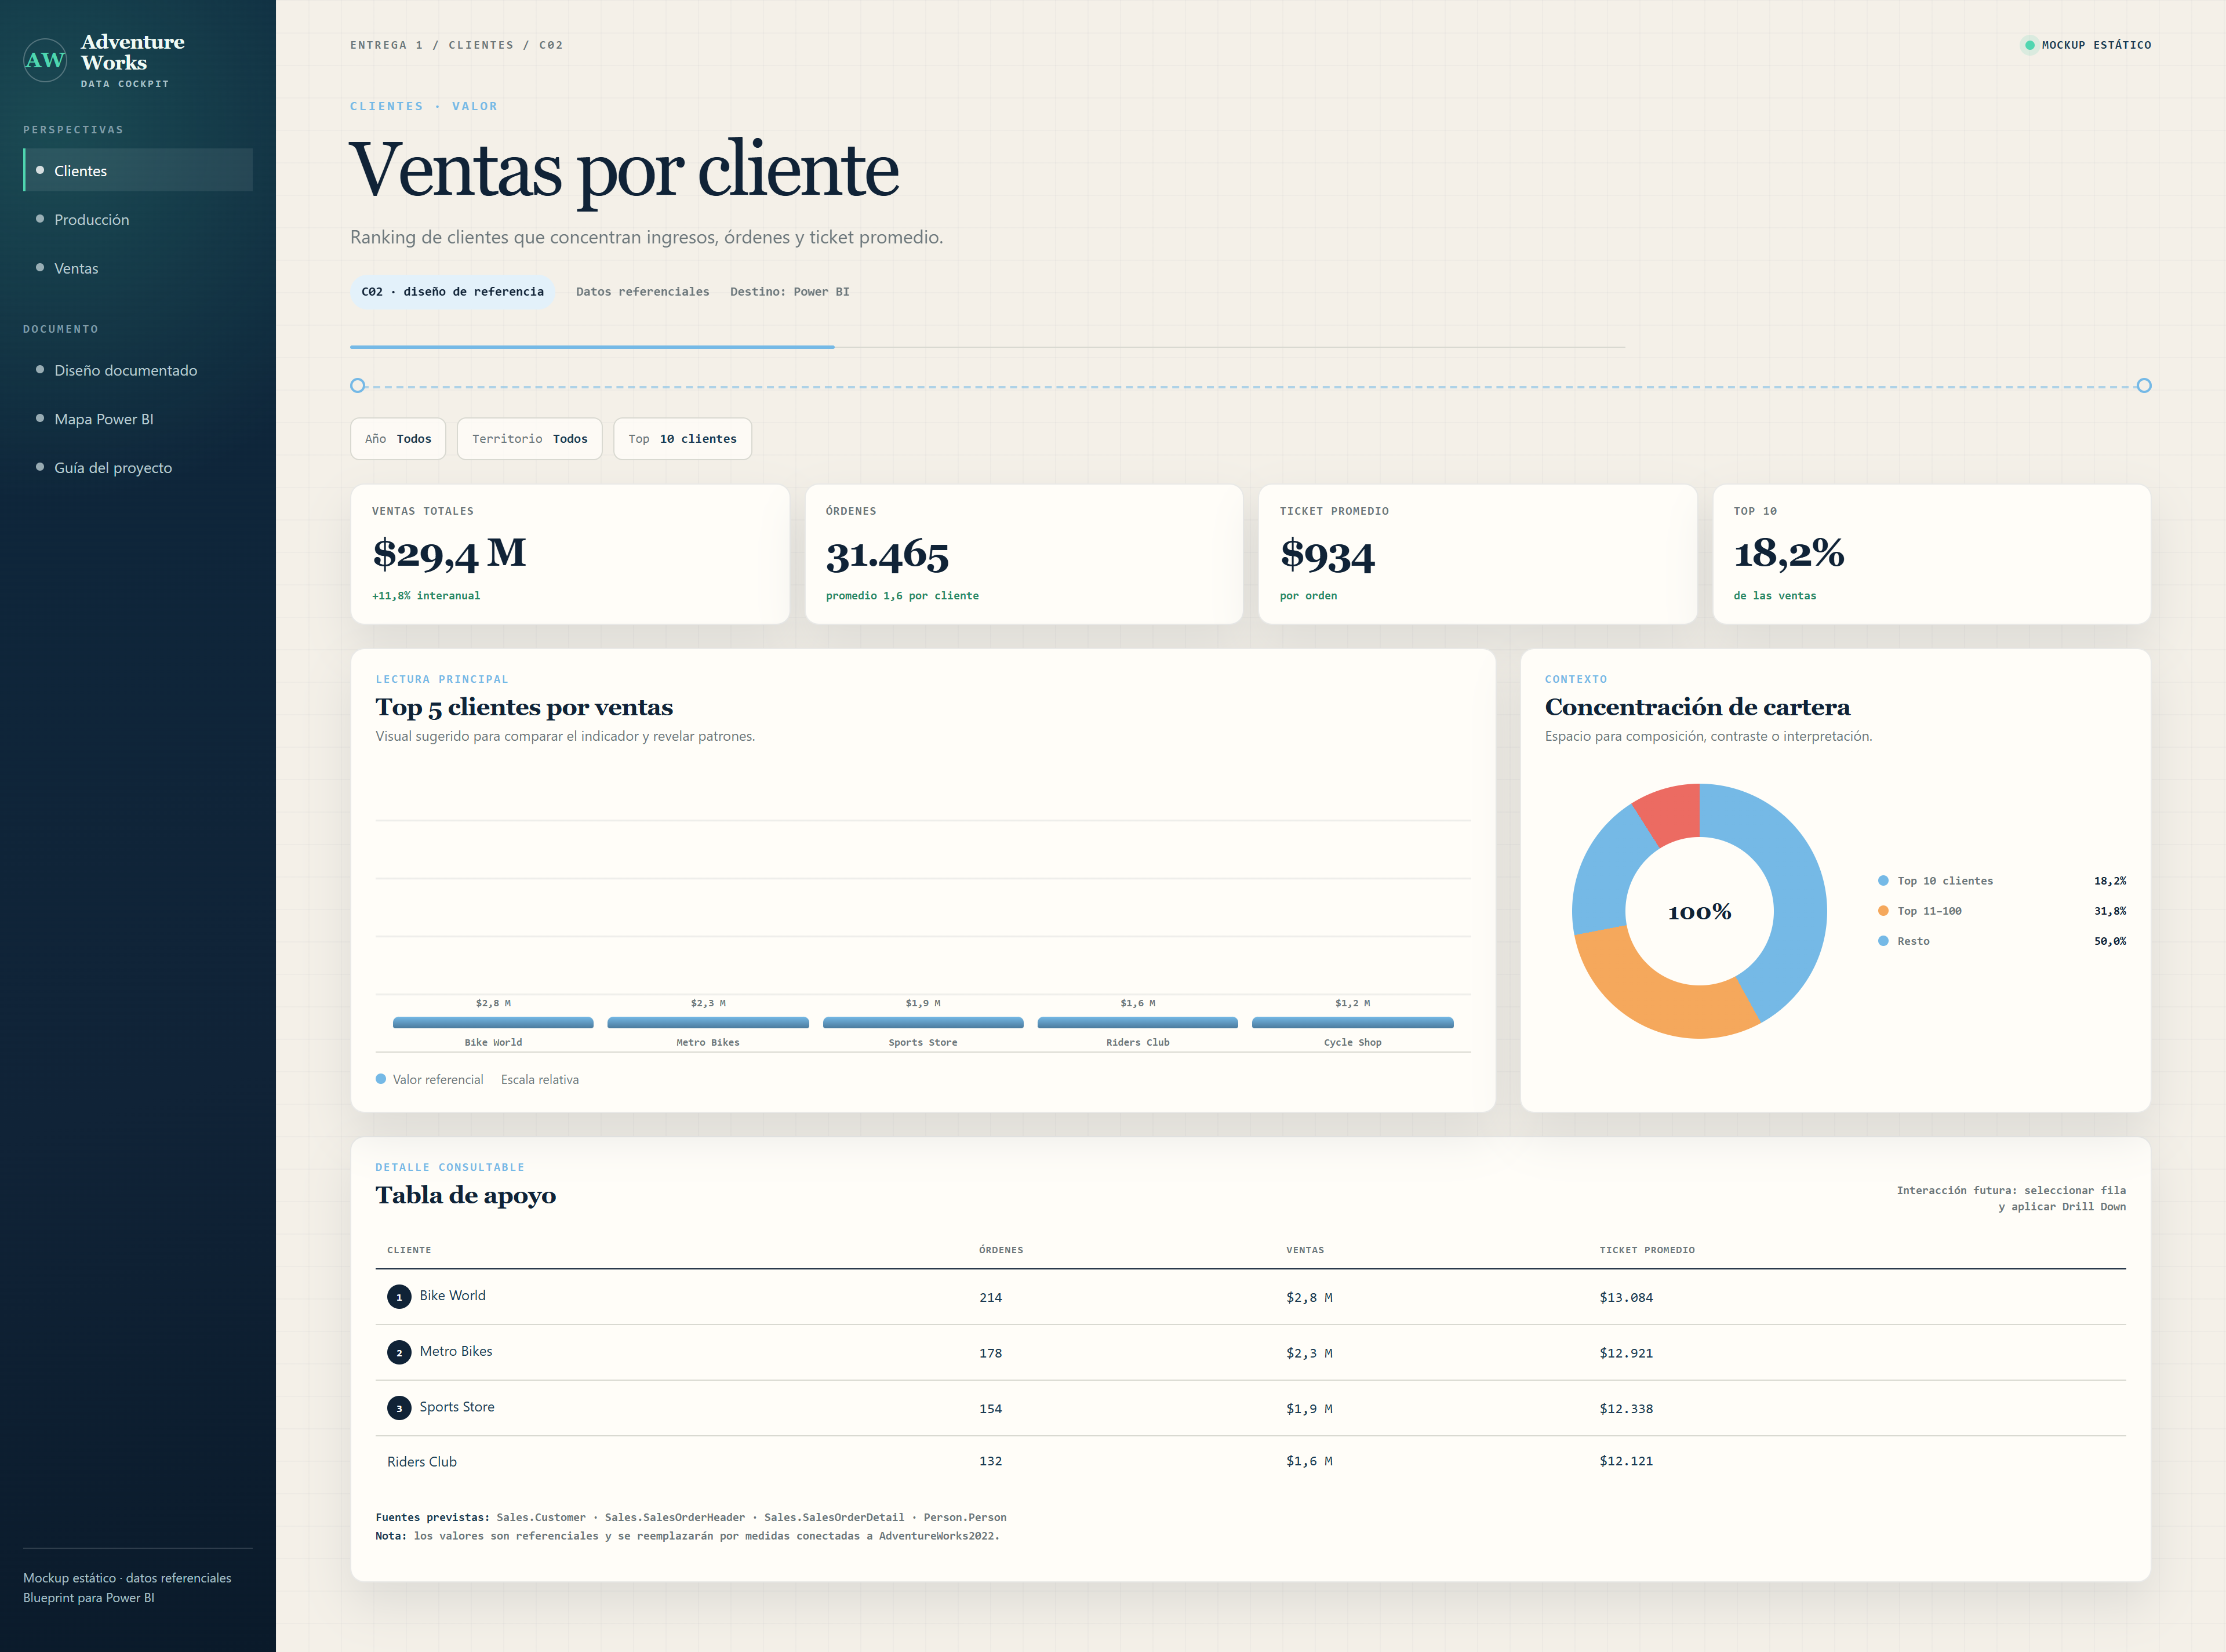
\includegraphics[width=0.84\textwidth]{mockup_clientes_02-ventas-por-cliente.png}
        \caption{Reporte C2: Ventas por cliente.}
    \end{figure}
    
    \clearpage
    \item \textbf{C3. Frecuencia y fidelidad:} Distinguir clientes frecuentes de ocasionales. Medirá órdenes promedio, clientes recurrentes y días entre compras.
    \nopagebreak
    \begin{figure}[H]
        \centering
        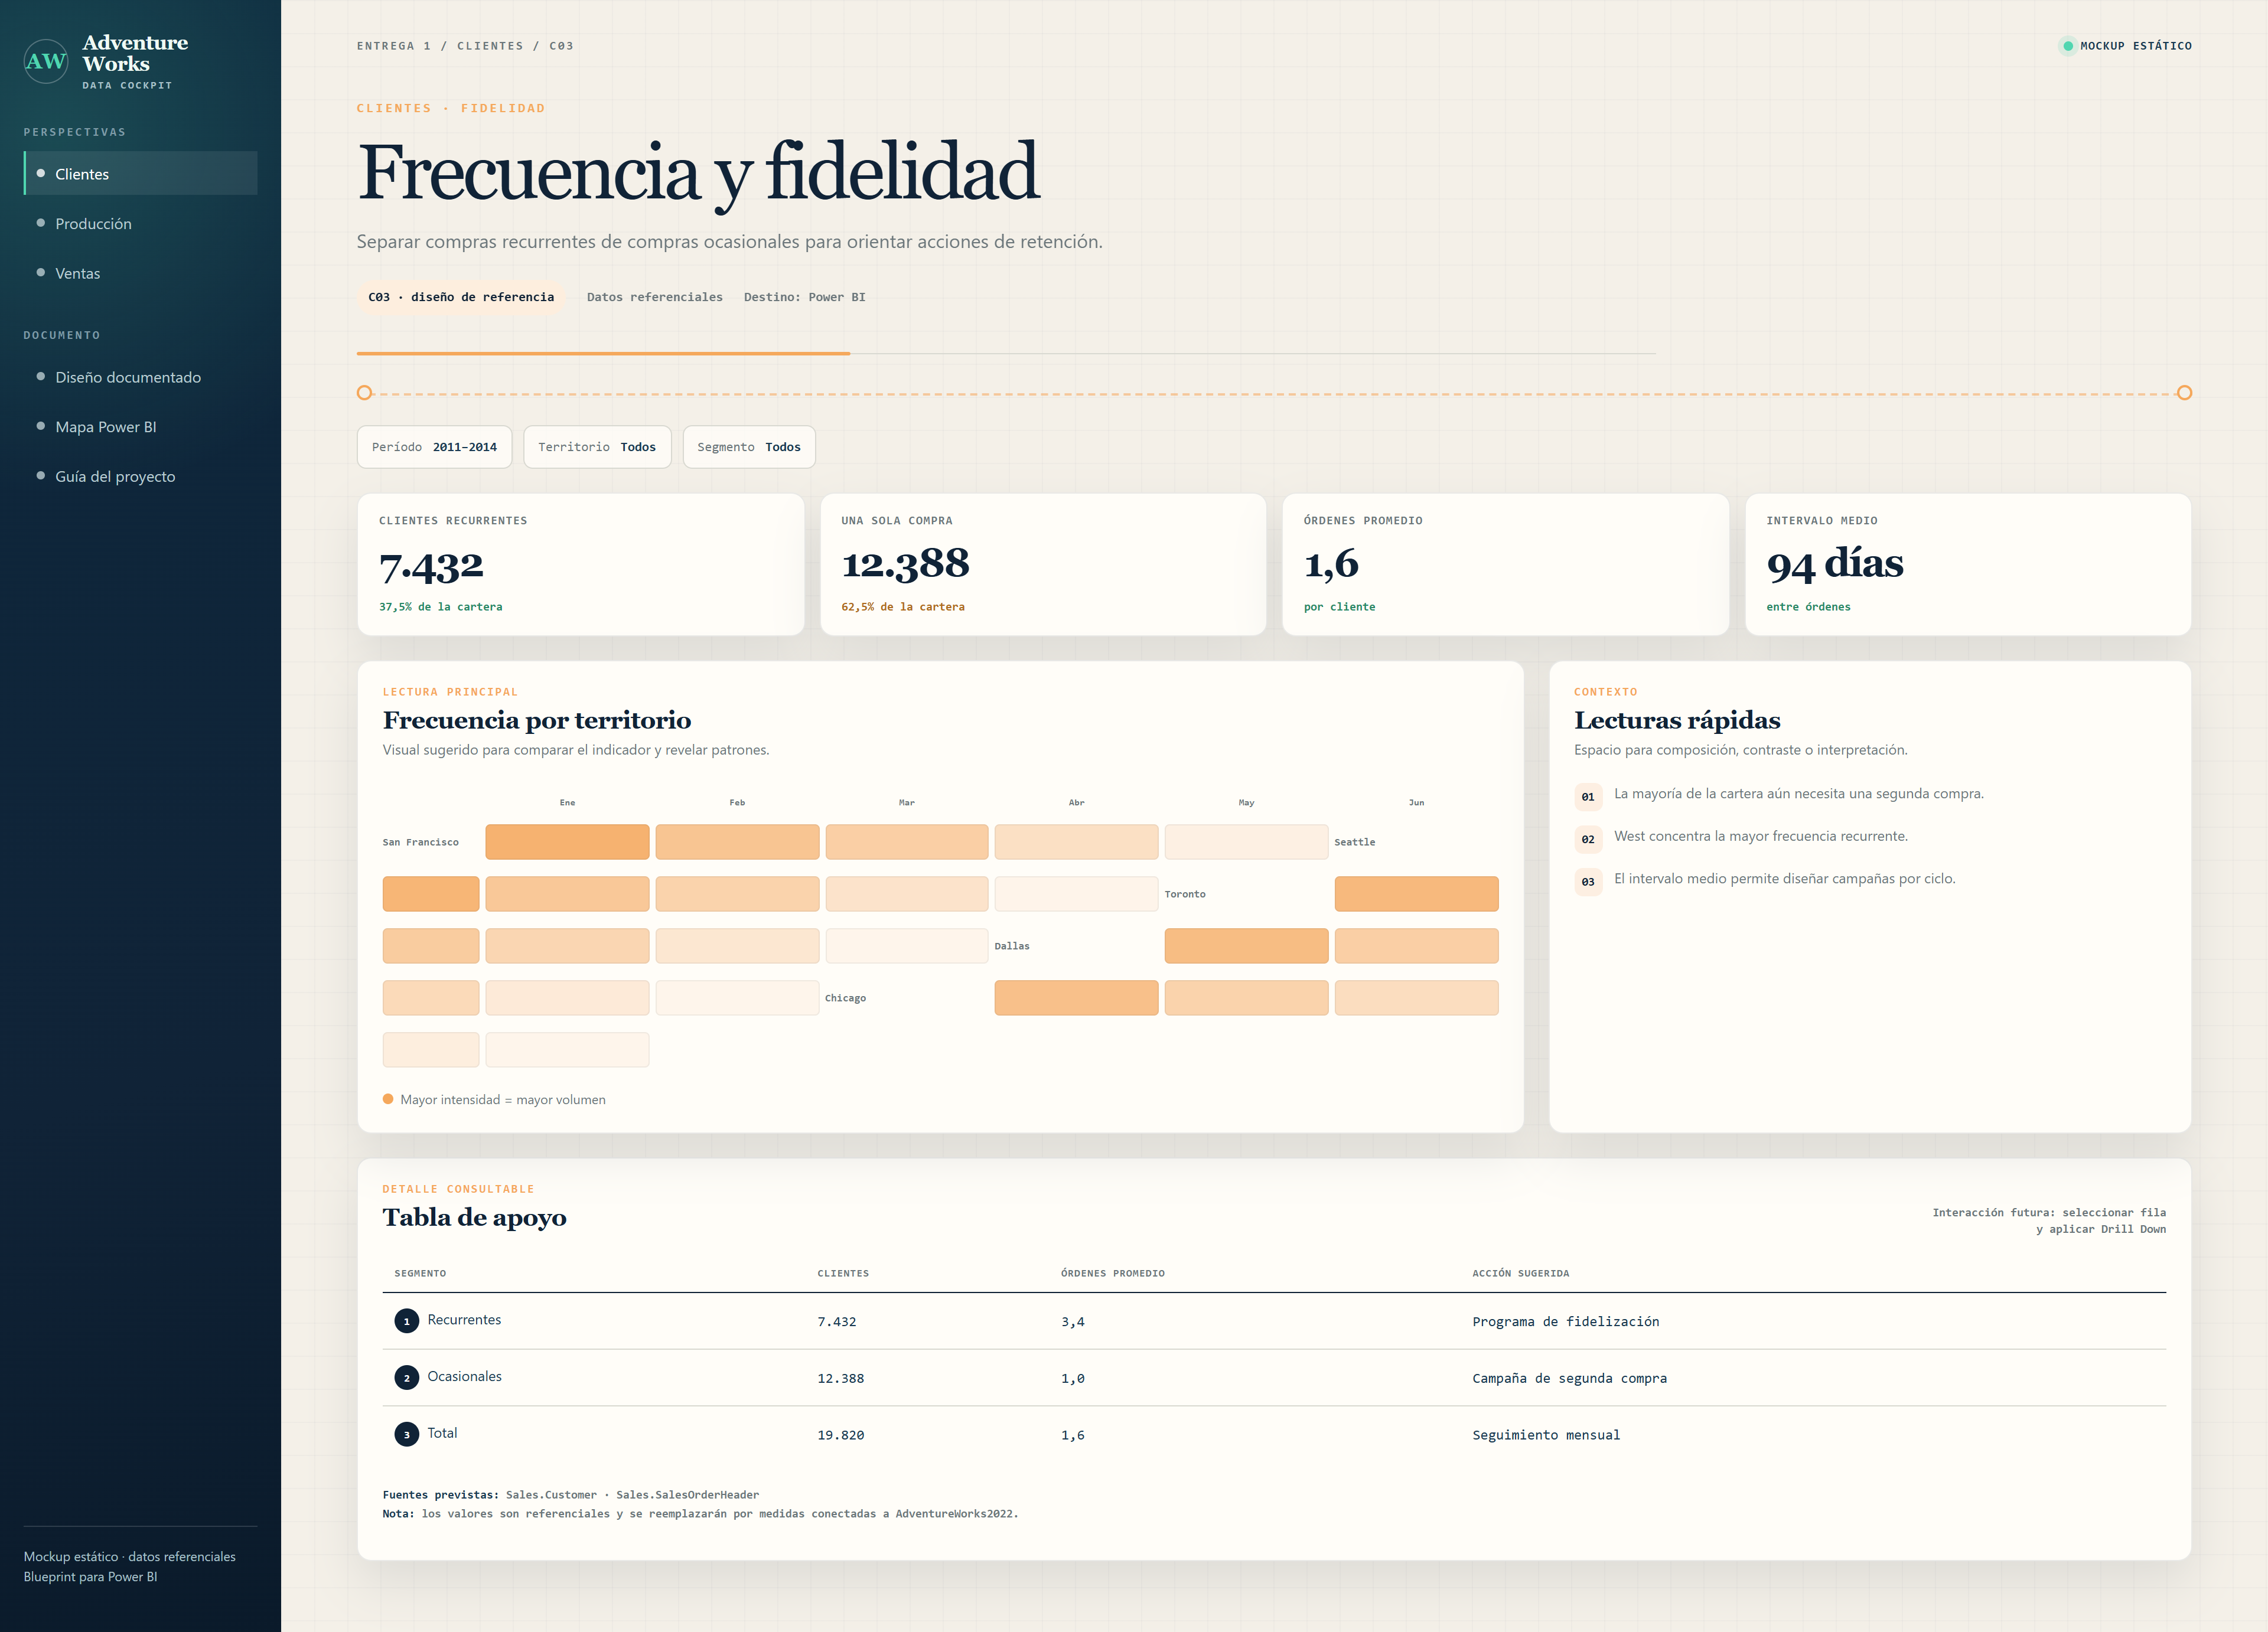
\includegraphics[width=0.84\textwidth]{mockup_clientes_03-frecuencia-fidelidad.png}
        \caption{Reporte C3: Frecuencia y fidelidad.}
    \end{figure}
    
    \clearpage
    \item \textbf{C4. Distribución geográfica:} Comparar la presencia de clientes por ubicación. Medirá clientes, órdenes y ventas por país y territorio.
    \nopagebreak
    \begin{figure}[H]
        \centering
        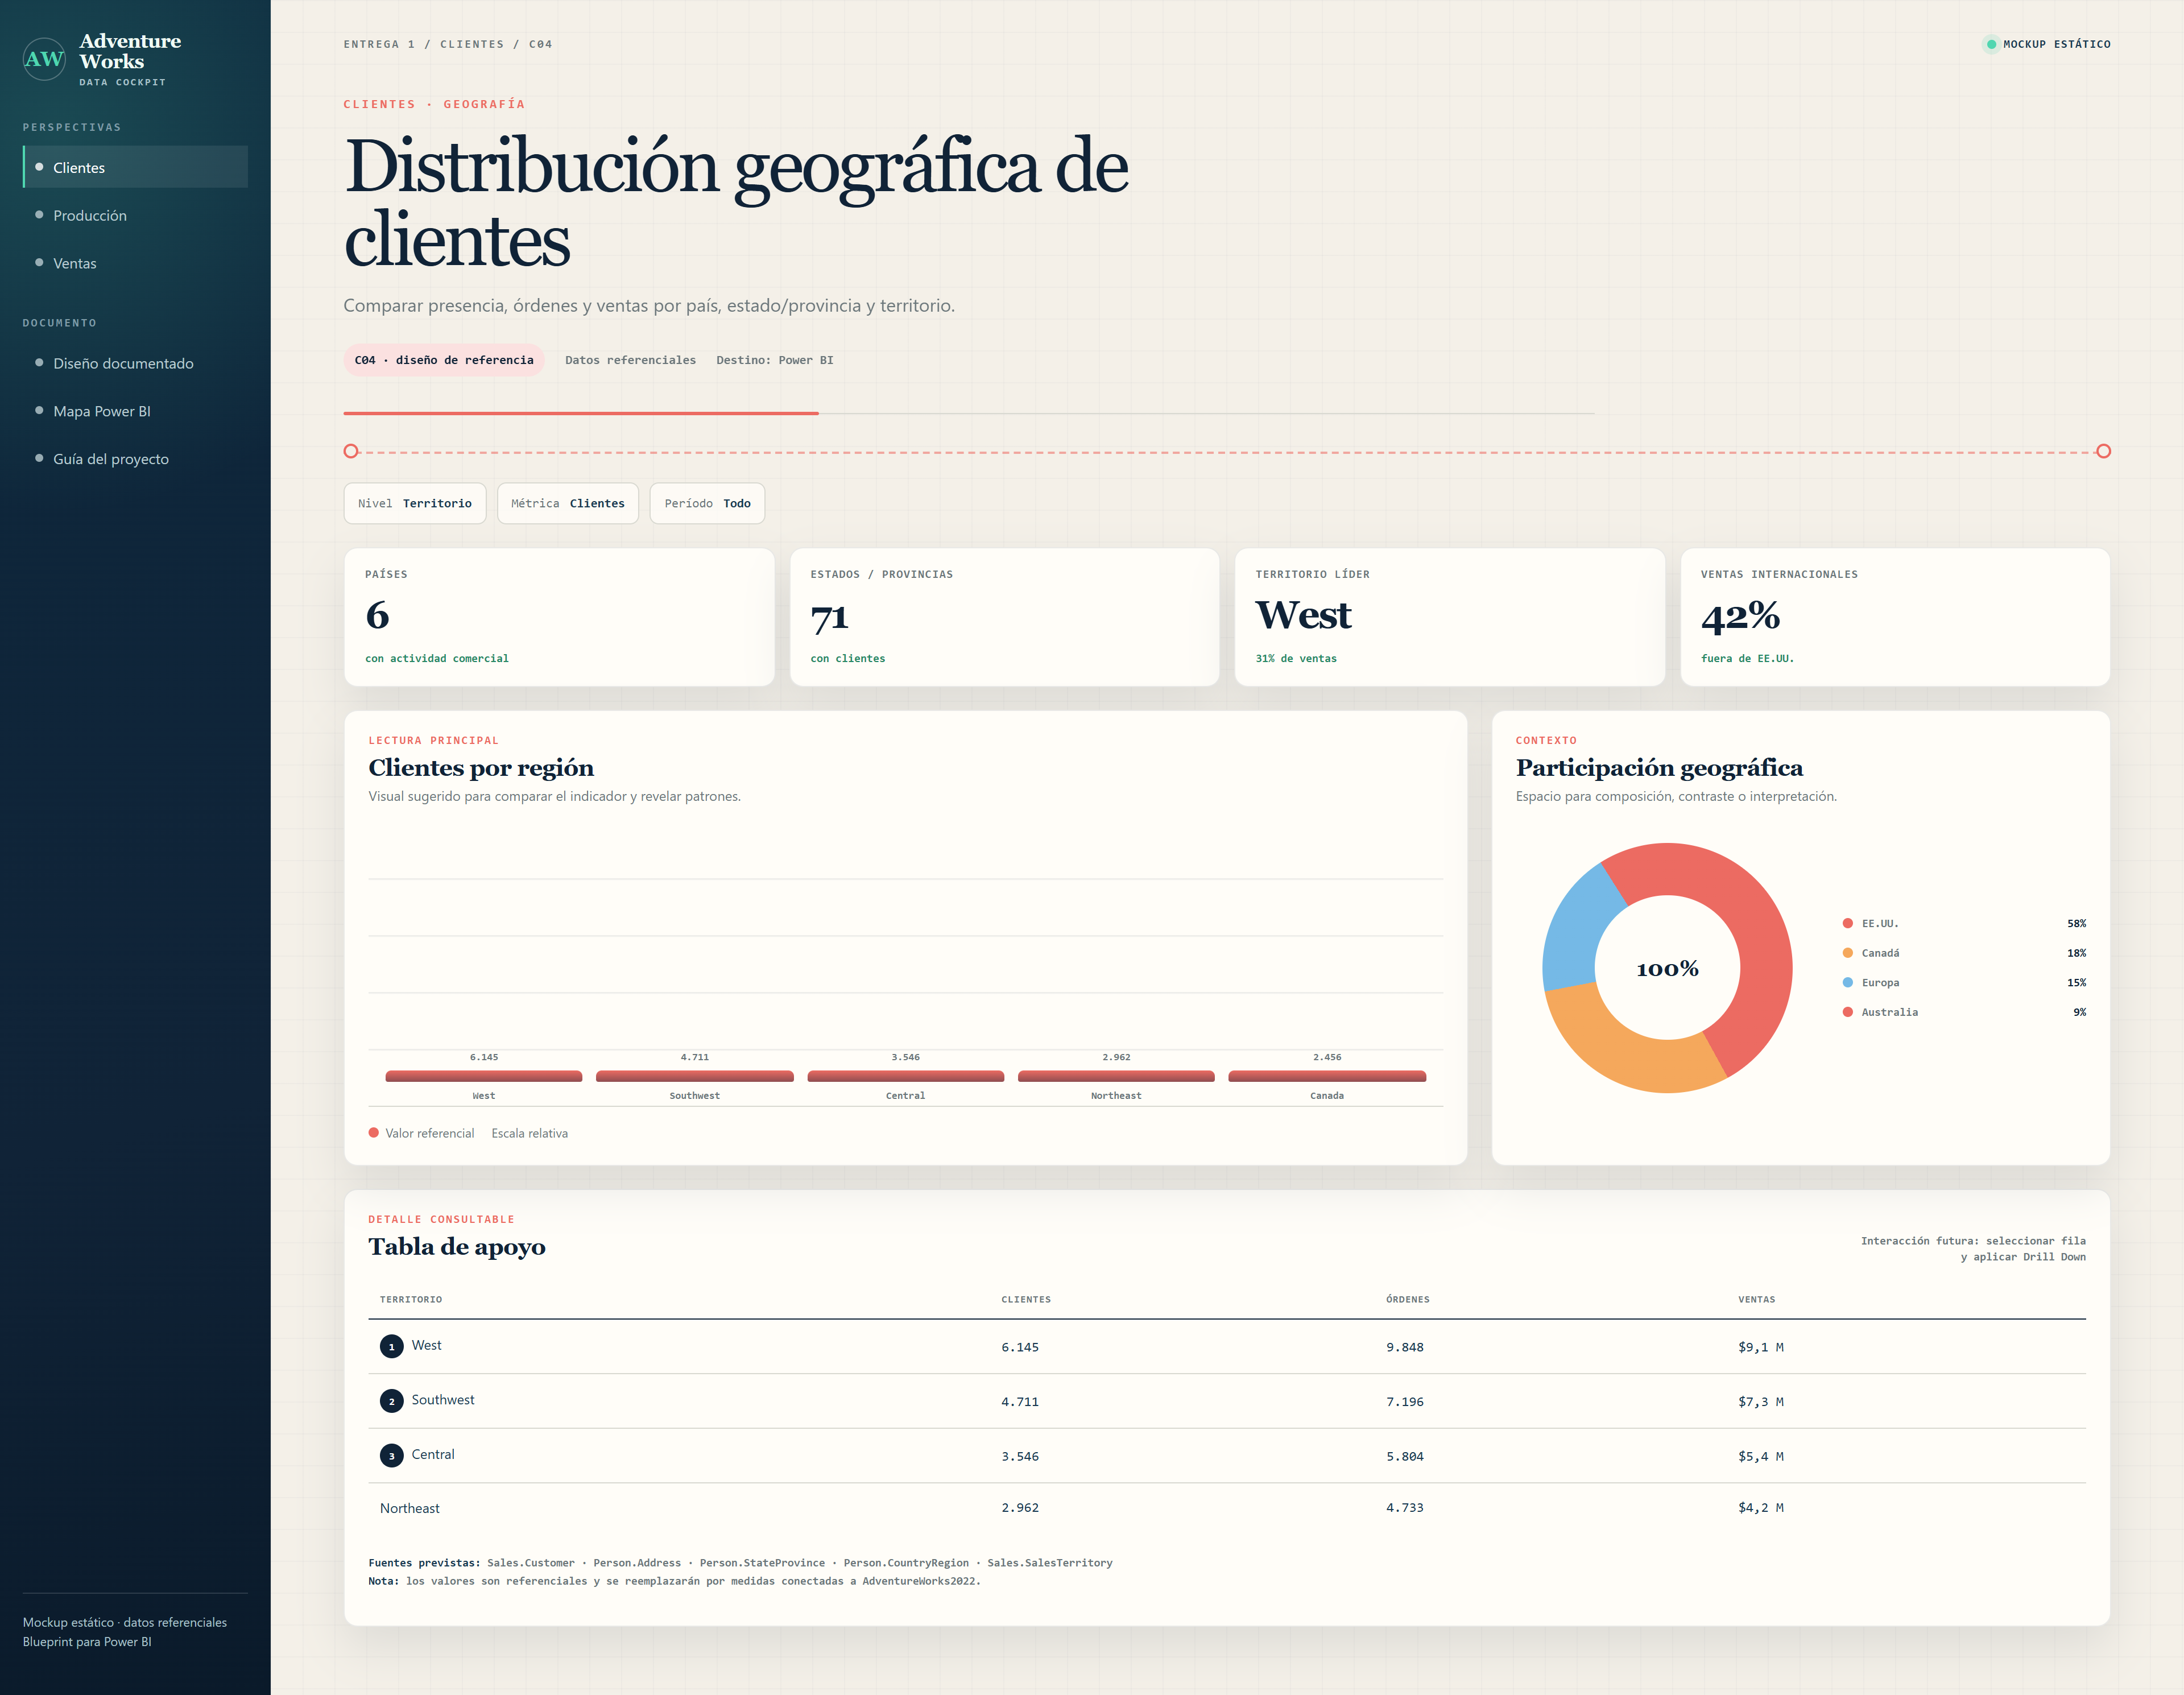
\includegraphics[width=0.84\textwidth]{mockup_clientes_04-distribucion-geografica.png}
        \caption{Reporte C4: Distribución geográfica.}
    \end{figure}
    
    \clearpage
    \item \textbf{C5. Clientes sin actividad reciente:} Detectar clientes para acciones de retención. Medirá clientes sin órdenes y tiempo de inactividad.
    \nopagebreak
    \begin{figure}[H]
        \centering
        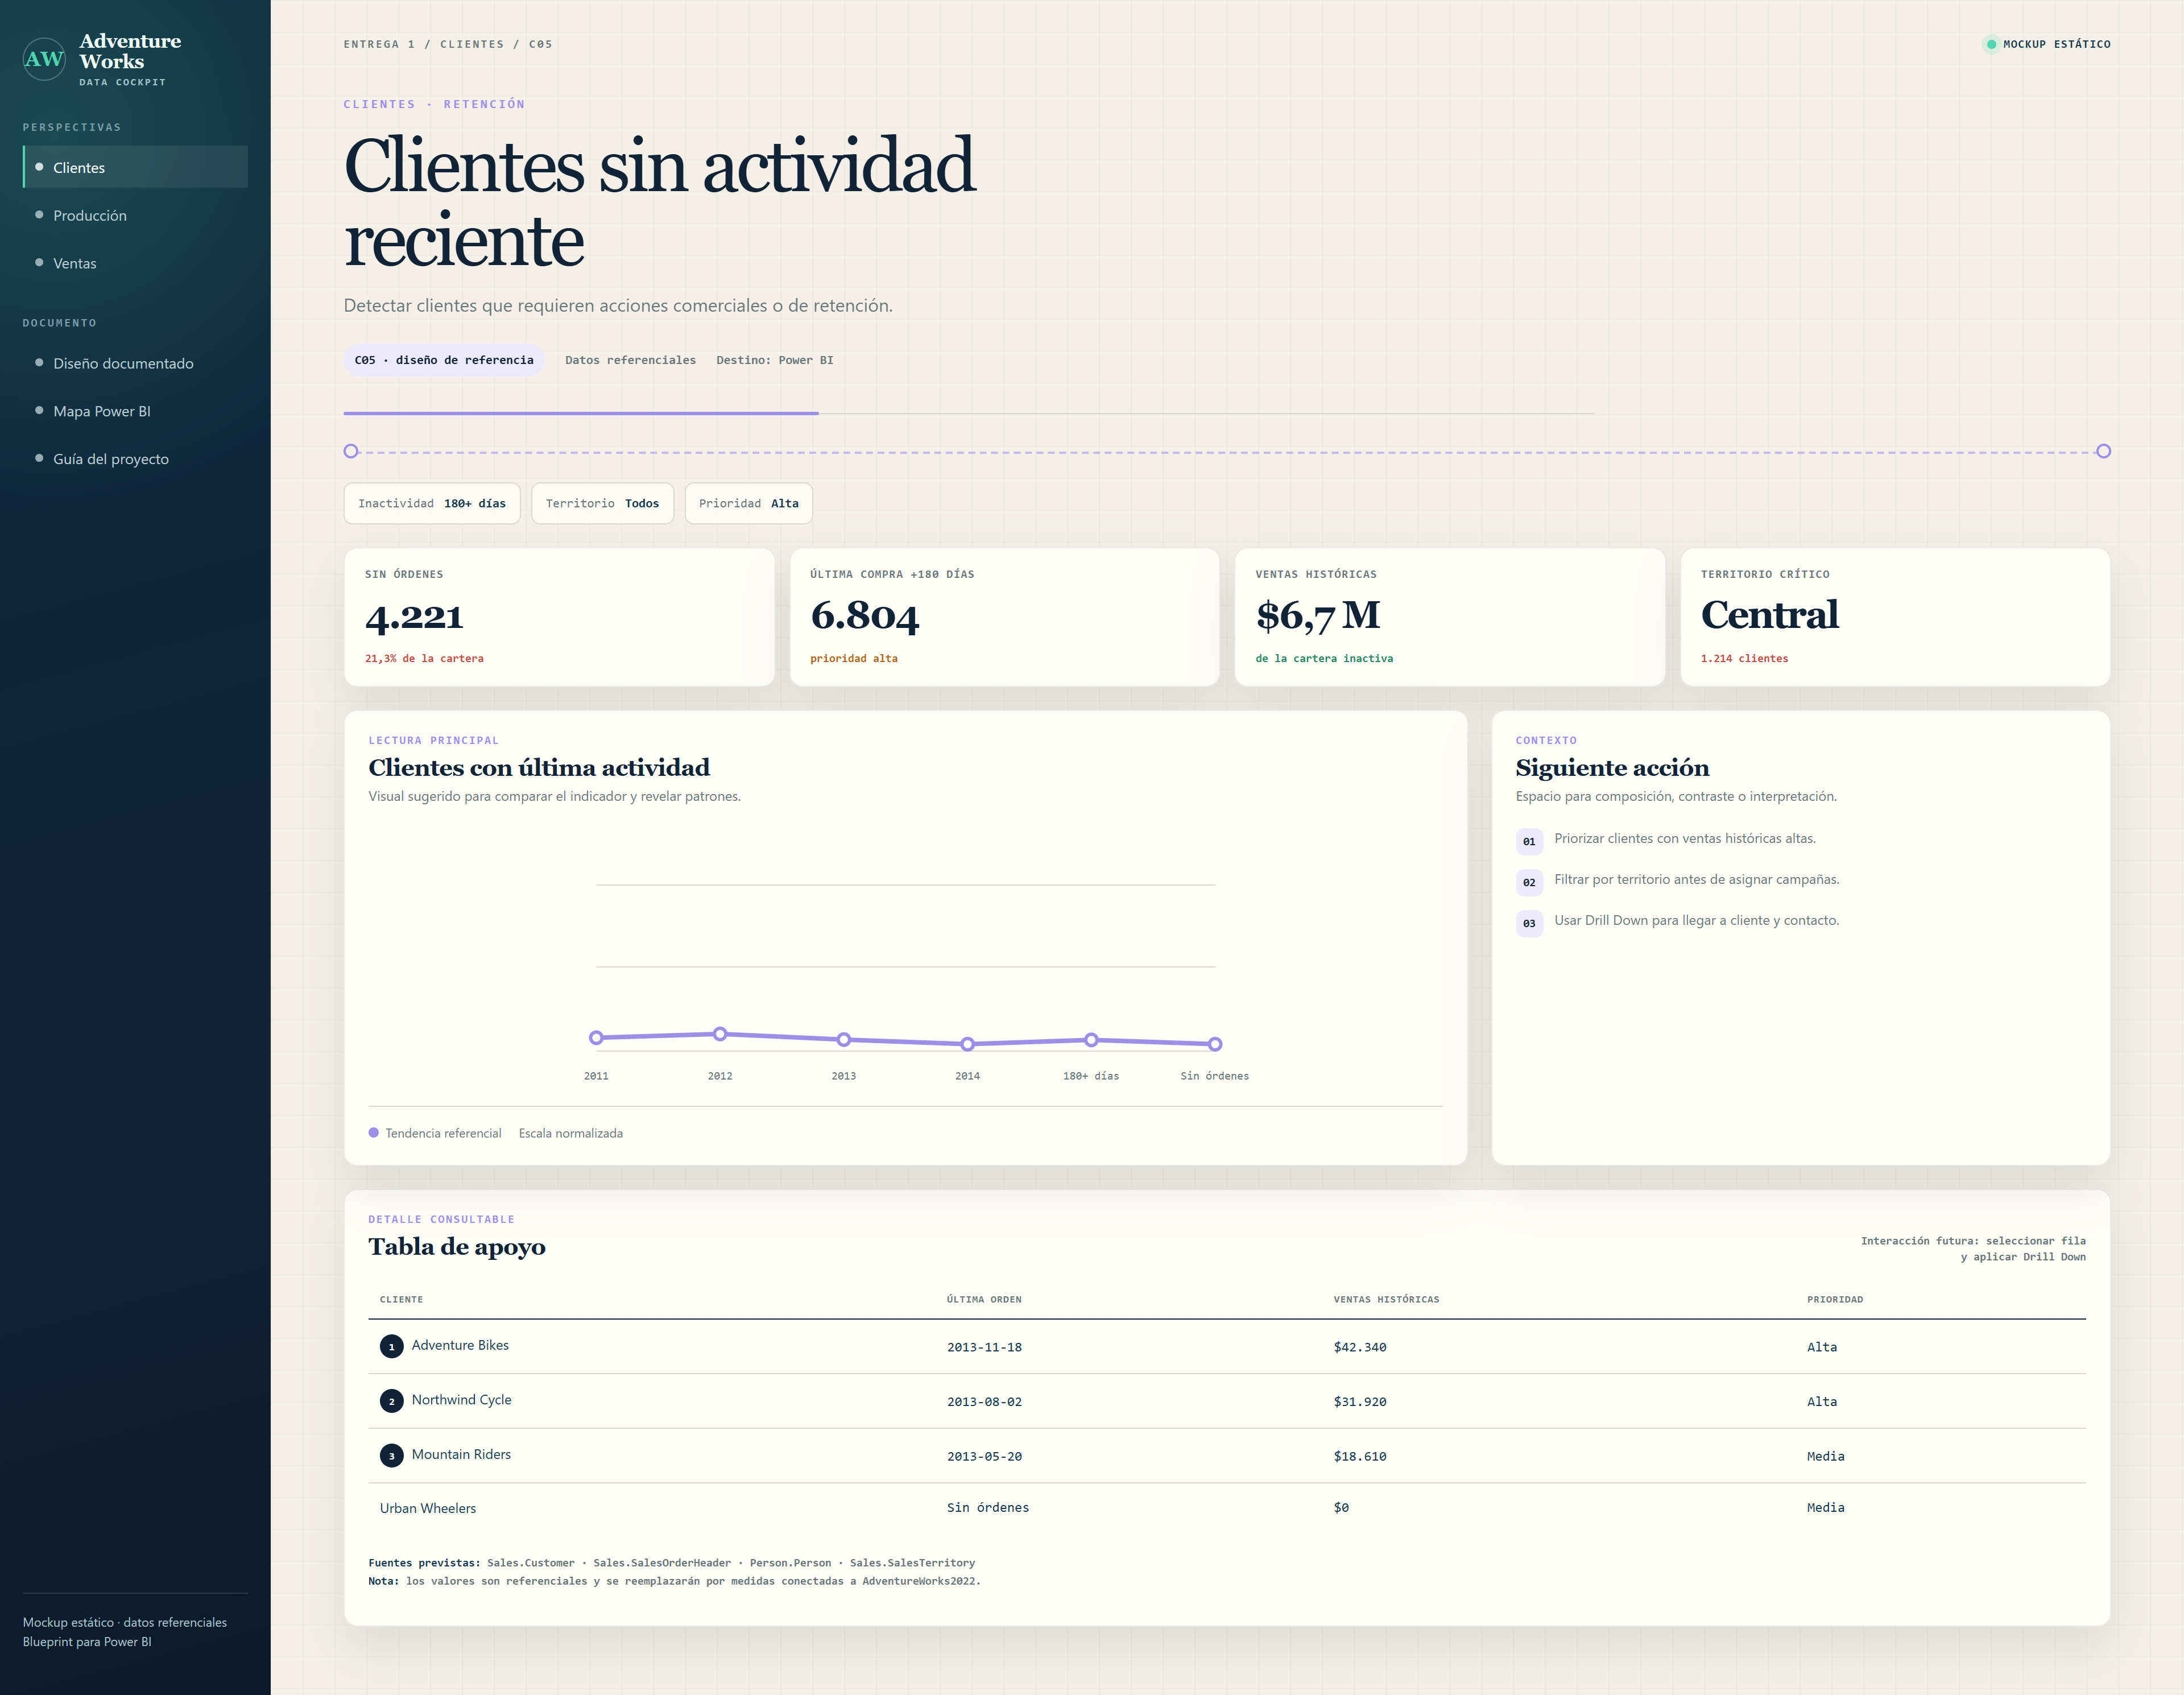
\includegraphics[width=0.84\textwidth]{mockup_clientes_05-clientes-inactivos.png}
        \caption{Reporte C5: Clientes sin actividad reciente.}
    \end{figure}
\end{enumerate}

\clearpage
%-----------------------------------------------------------------------

\subsection{Perspectiva de Procesos (Producción)}
Se proponen los siguientes 5 reportes:
\begin{enumerate}
    \item \textbf{P1. Producción por producto y categoría:} Observar la actividad productiva. Medirá órdenes de trabajo, unidades a producir y tasa de rechazo.
    \nopagebreak
    \begin{figure}[H]
        \centering
        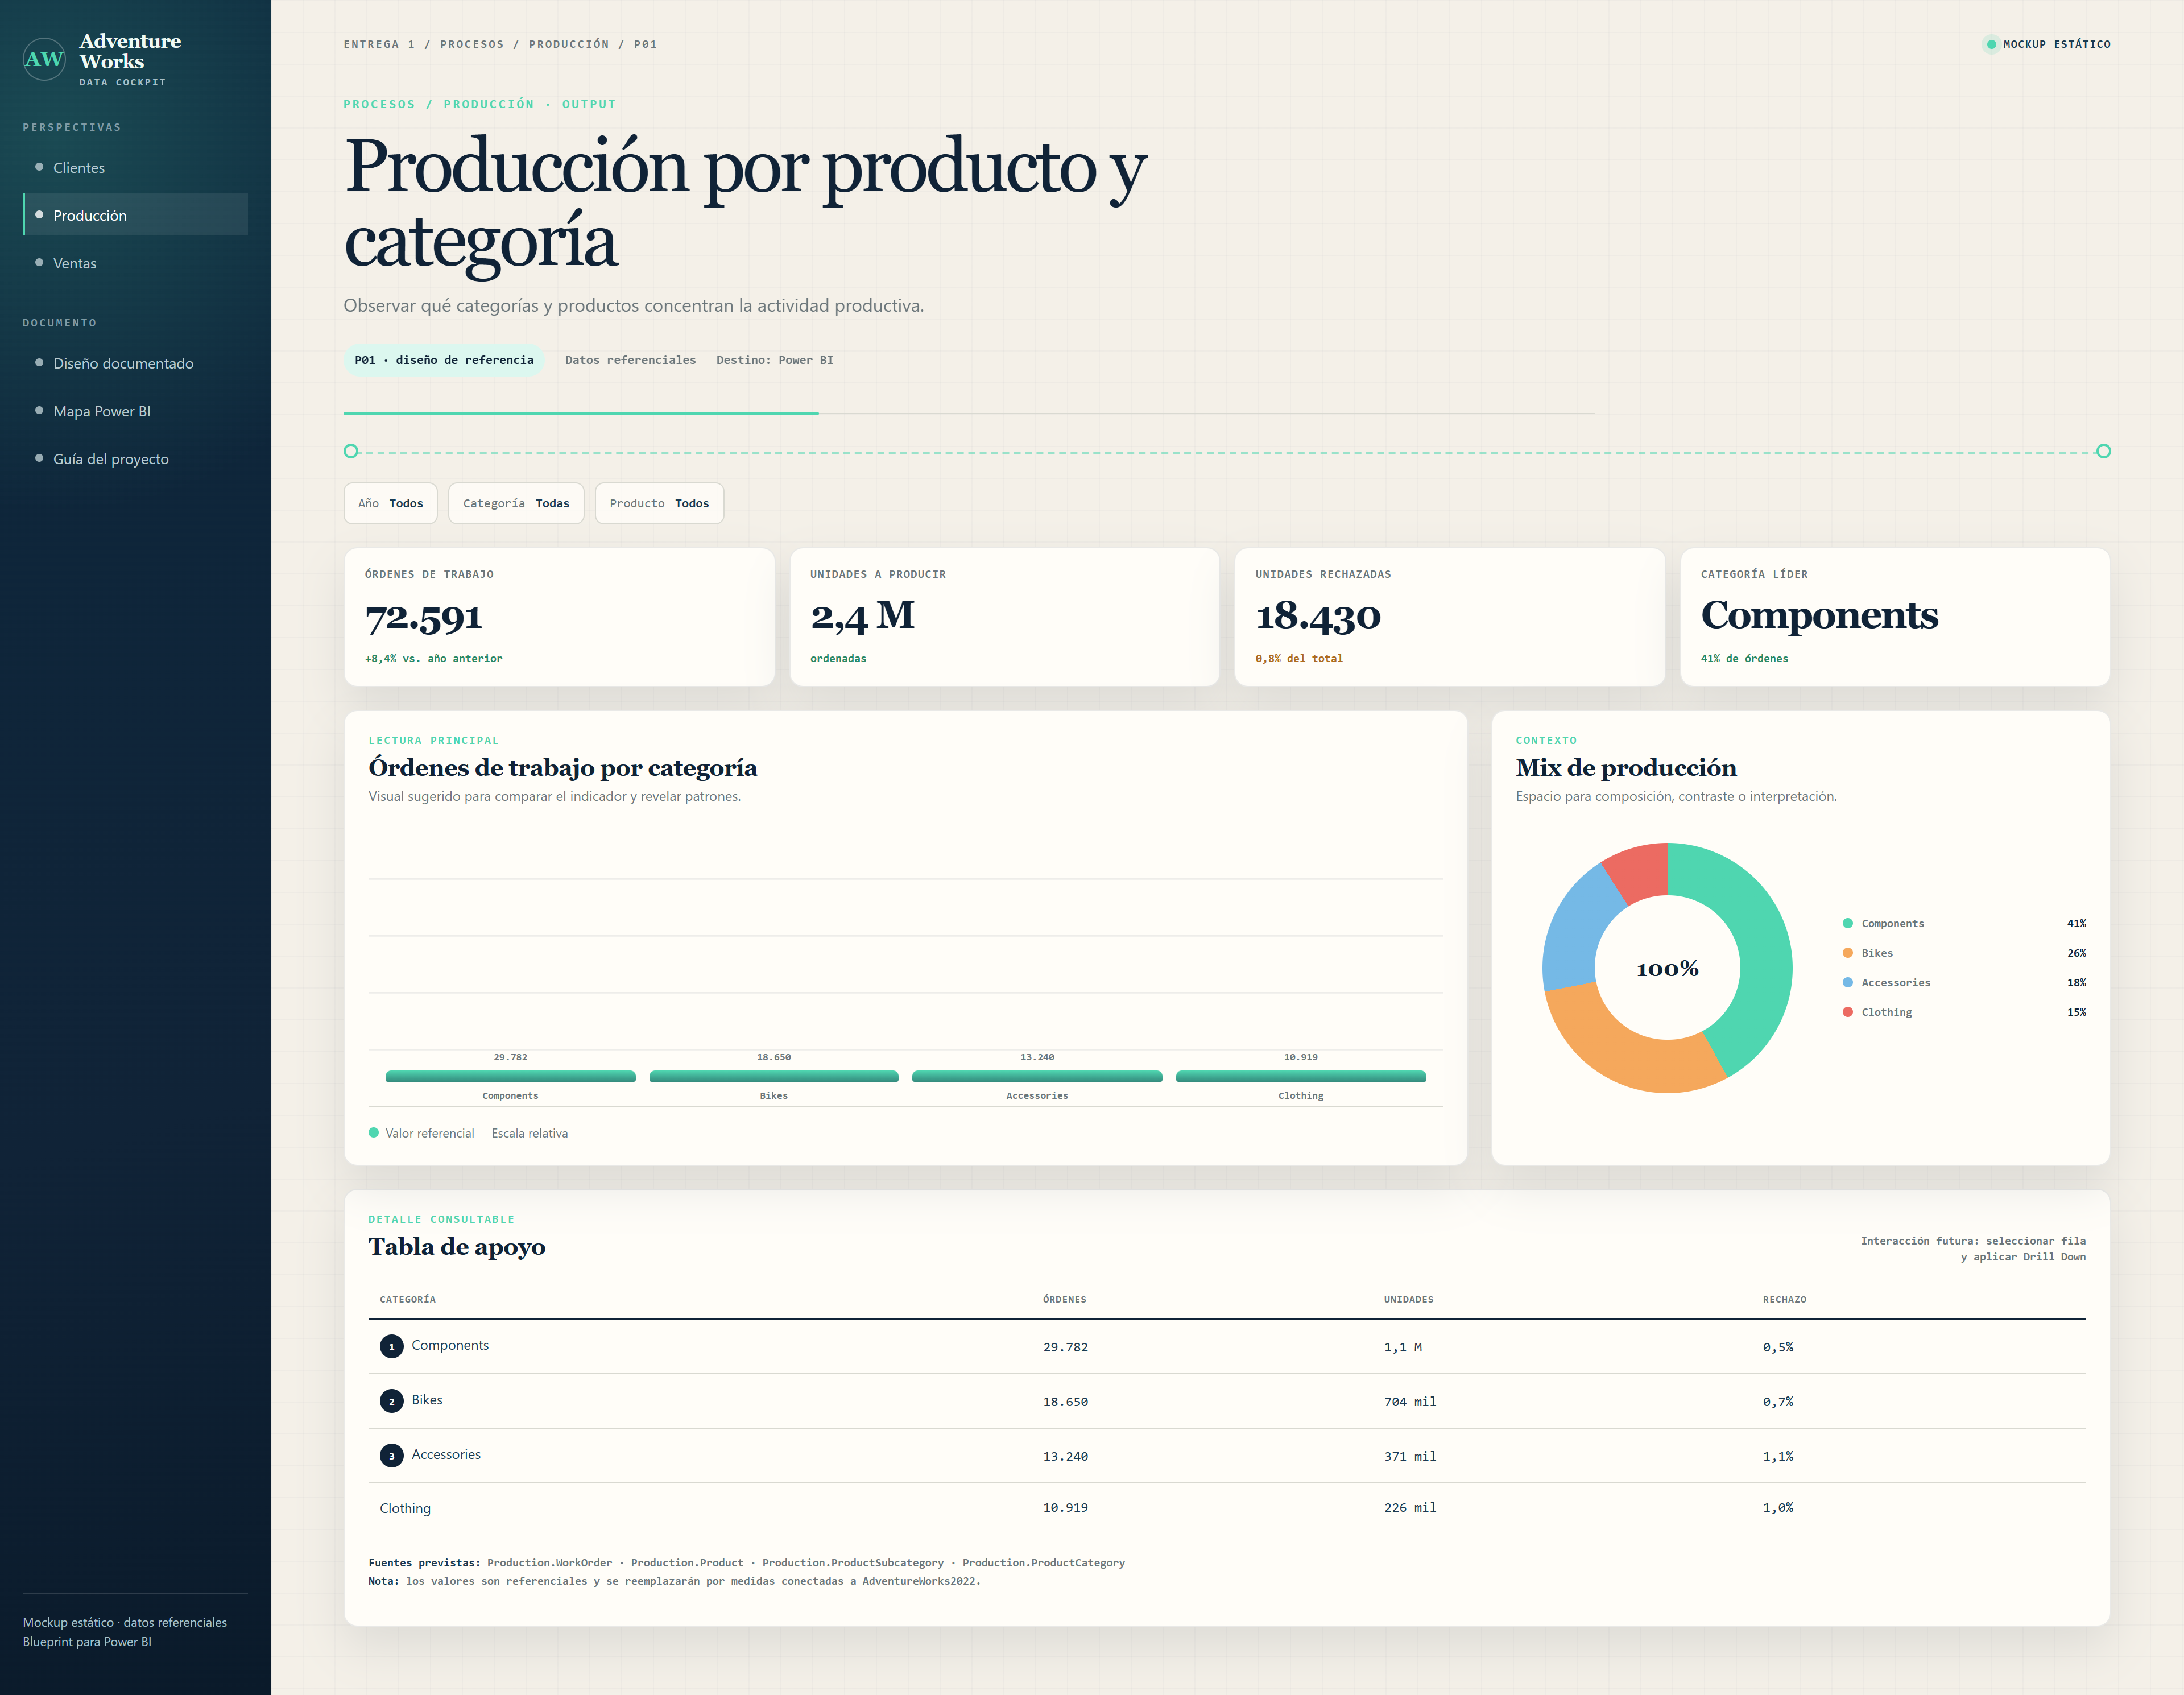
\includegraphics[width=0.82\textwidth]{mockup_produccion_01-produccion-producto.png}
        \caption{Reporte P1: Producción por producto y categoría.}
    \end{figure}
    
    \clearpage
    \item \textbf{P2. Inventario por ubicación:} Conocer la disponibilidad de productos. Medirá unidades en inventario y productos por ubicación.
    \nopagebreak
    \begin{figure}[H]
        \centering
        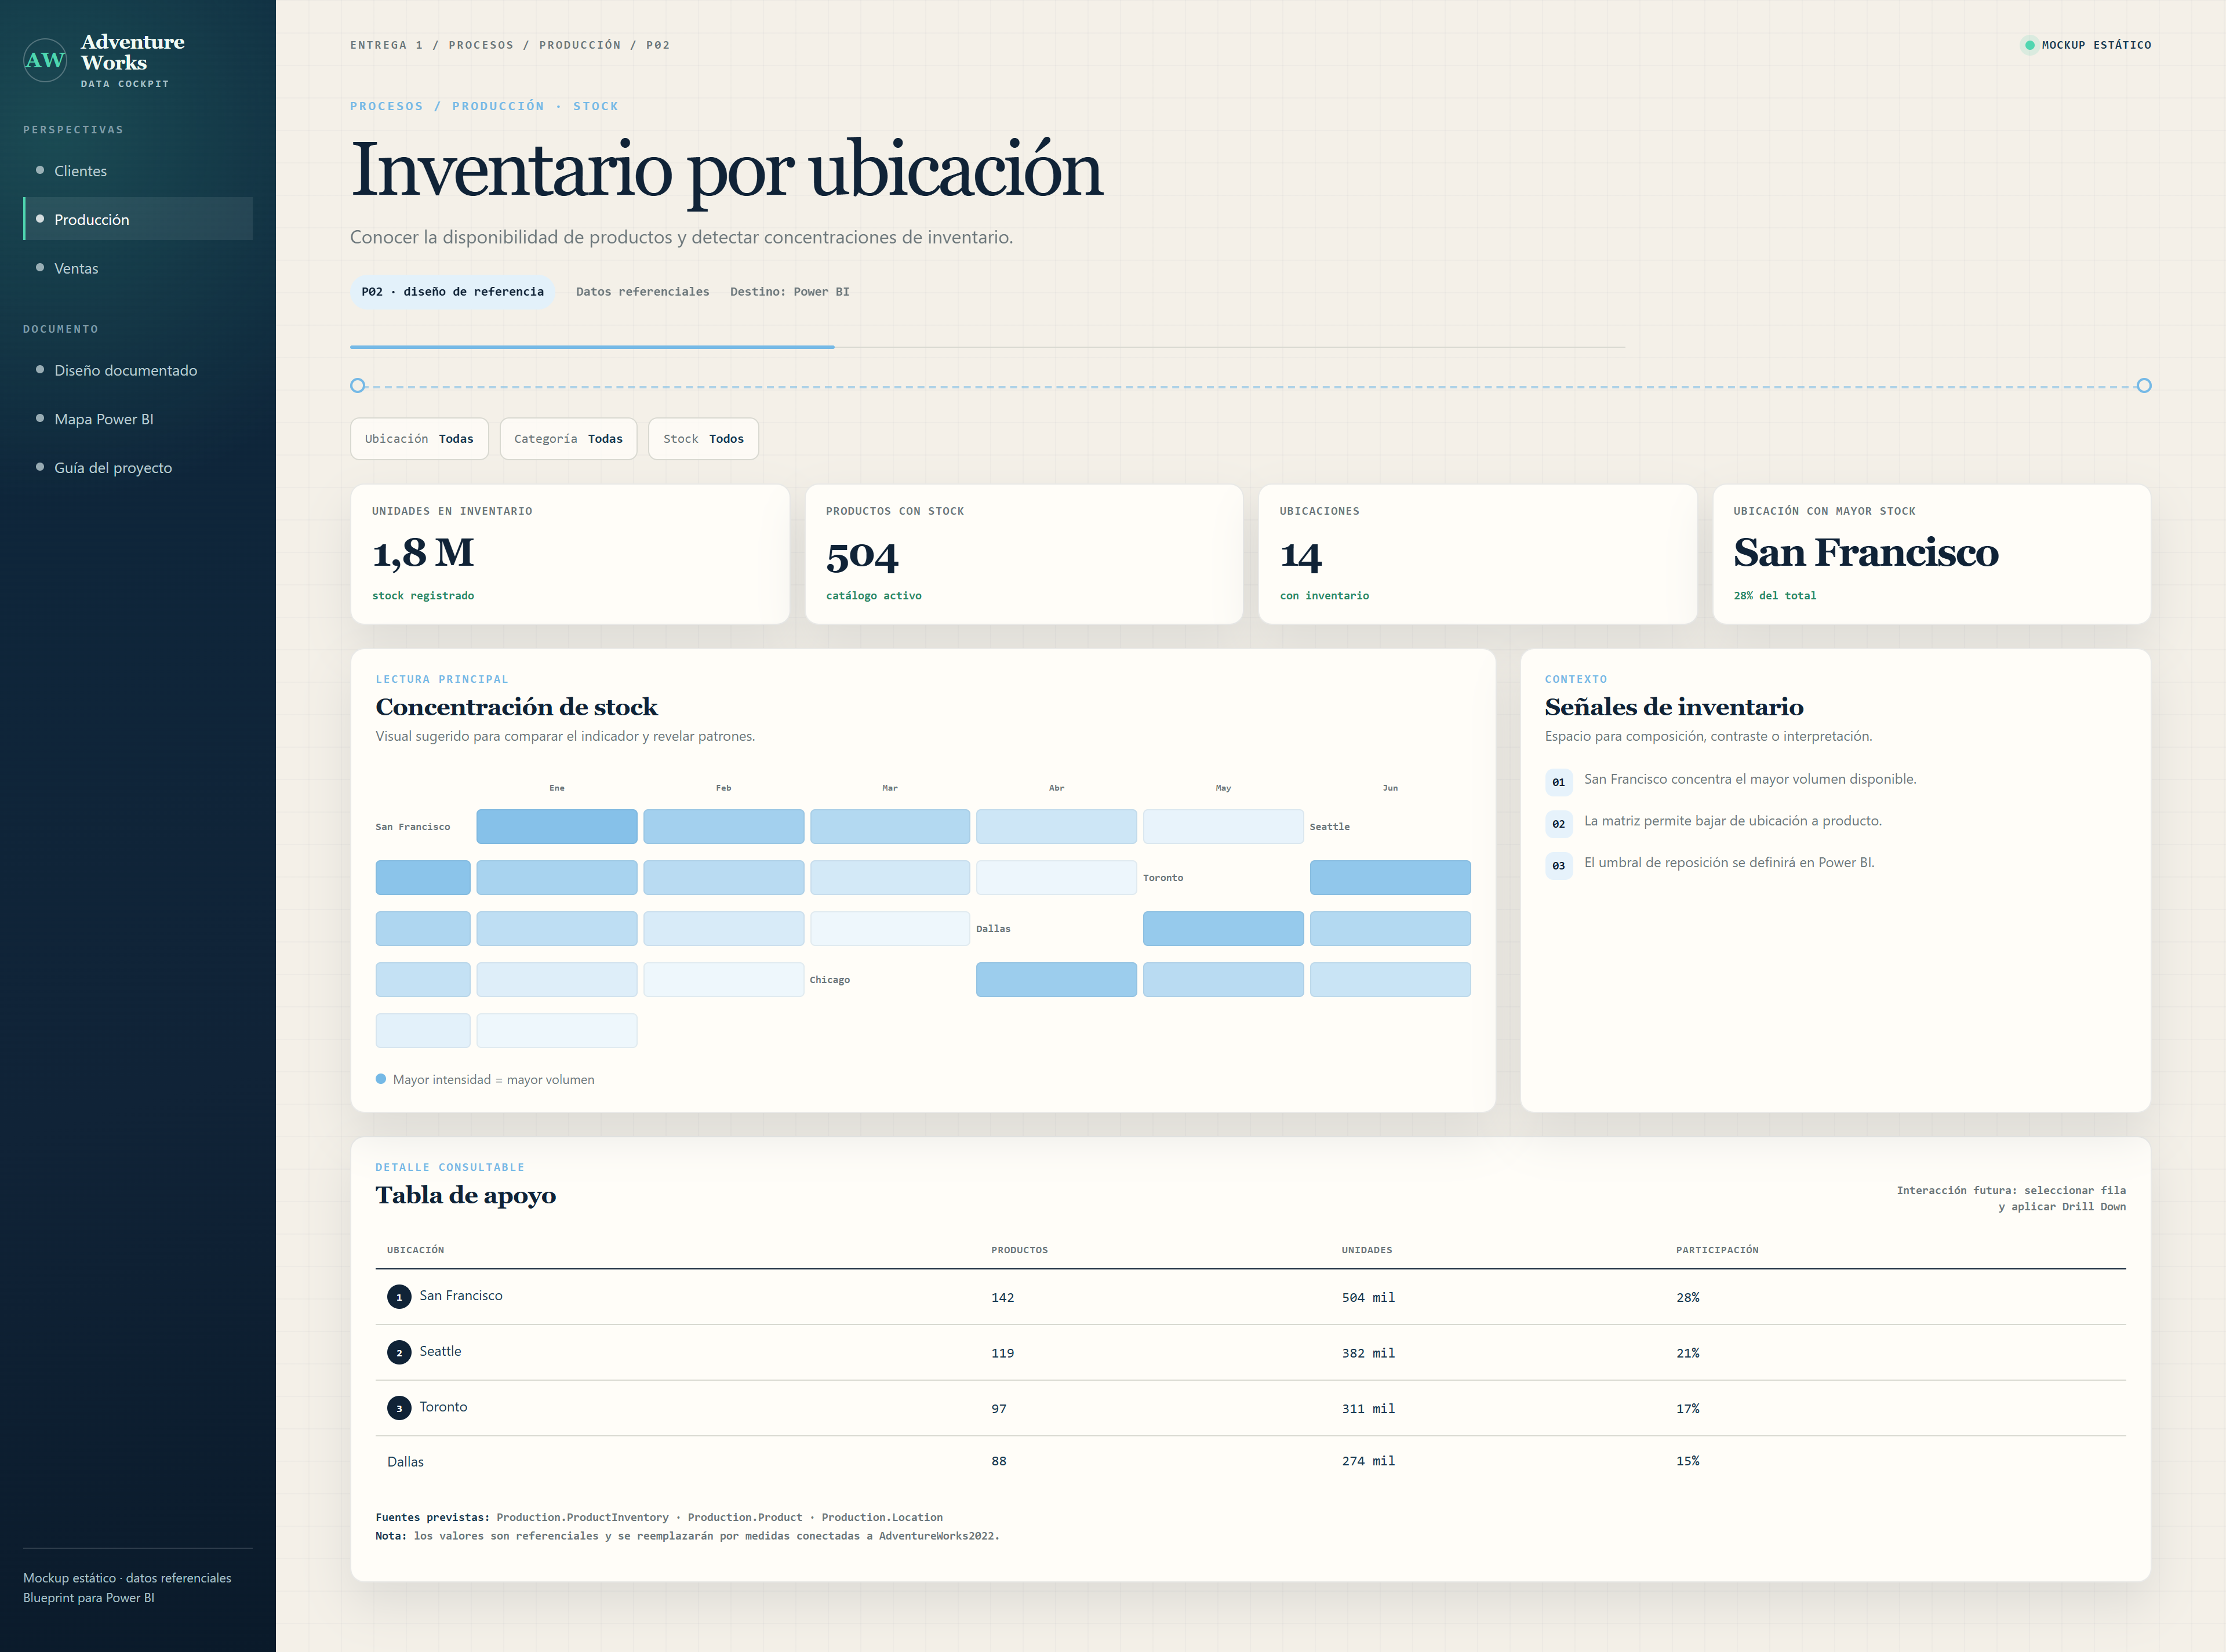
\includegraphics[width=0.84\textwidth]{mockup_produccion_02-inventario-ubicacion.png}
        \caption{Reporte P2: Inventario por ubicación.}
    \end{figure}
    
    \clearpage
    \item \textbf{P3. Cumplimiento de órdenes de trabajo:} Medir cumplimiento de plazos. Medirá órdenes terminadas, atrasadas y días de ejecución.
    \nopagebreak
    \begin{figure}[H]
        \centering
        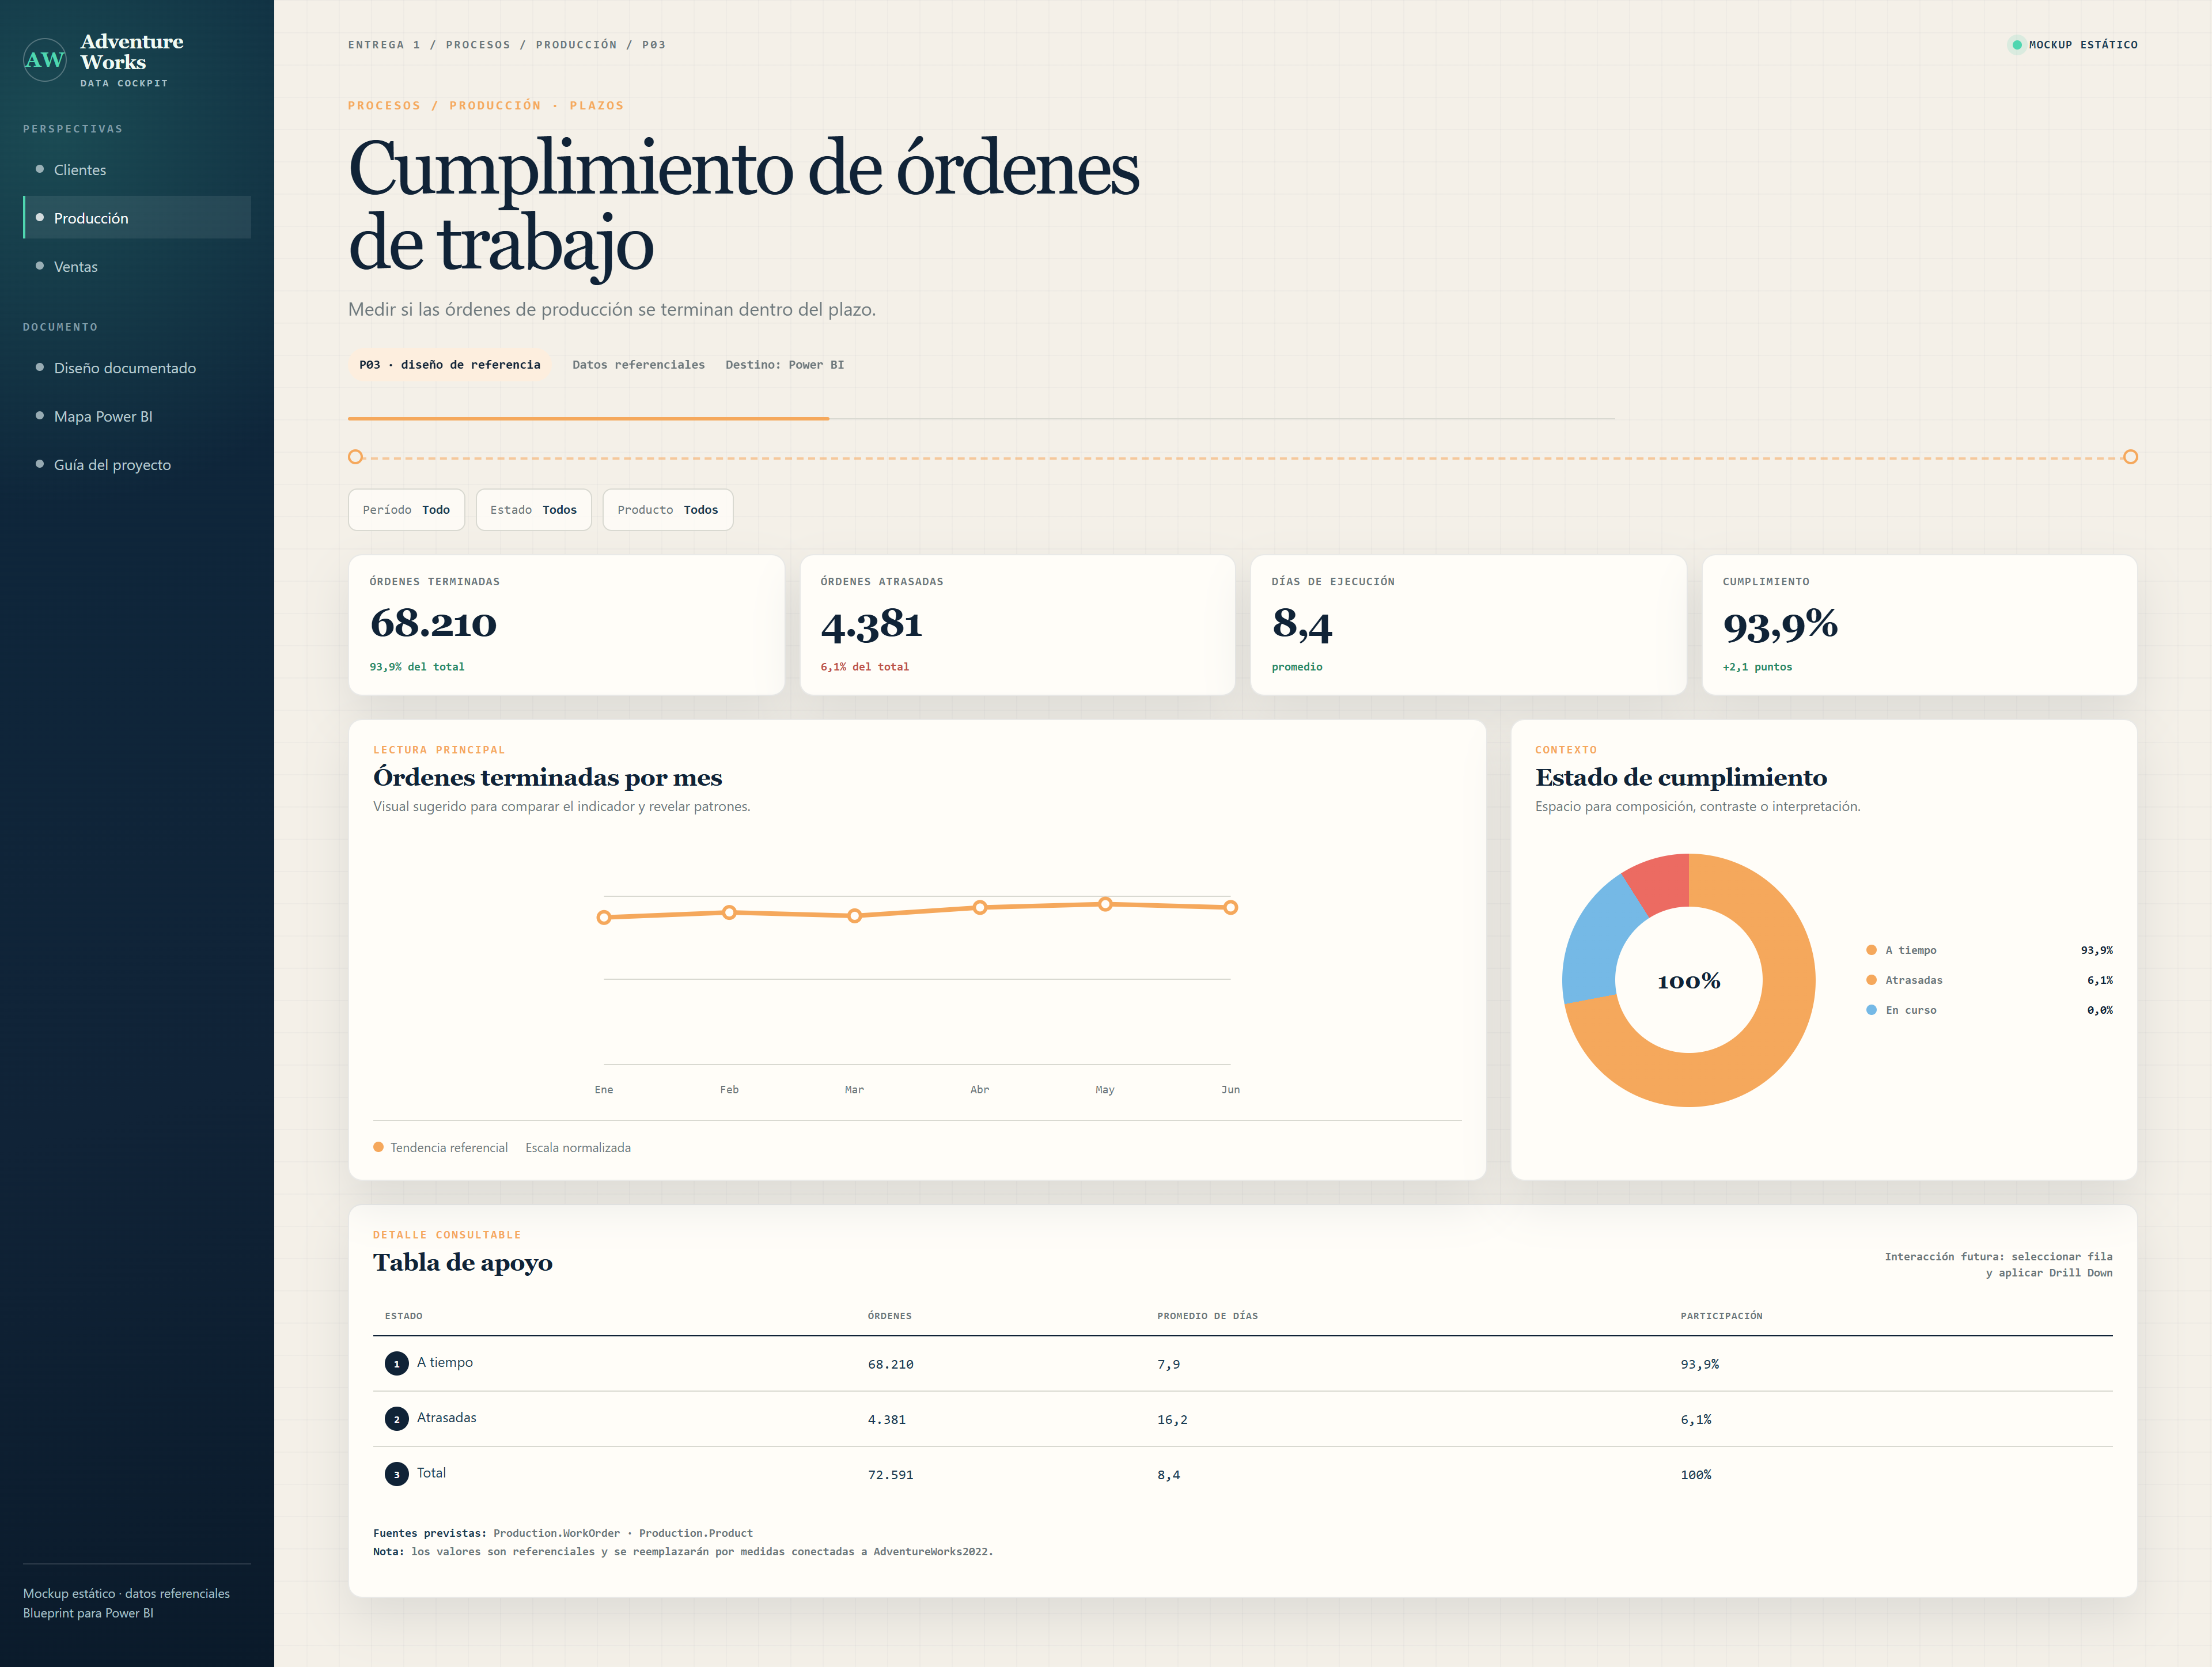
\includegraphics[width=0.84\textwidth]{mockup_produccion_03-cumplimiento-ordenes.png}
        \caption{Reporte P3: Cumplimiento de órdenes de trabajo.}
    \end{figure}
    
    \clearpage
    \item \textbf{P4. Eficiencia de las rutas productivas:} Comparar horas y costos planificados vs. reales. Medirá desviaciones de horas y costos.
    \nopagebreak
    \begin{figure}[H]
        \centering
        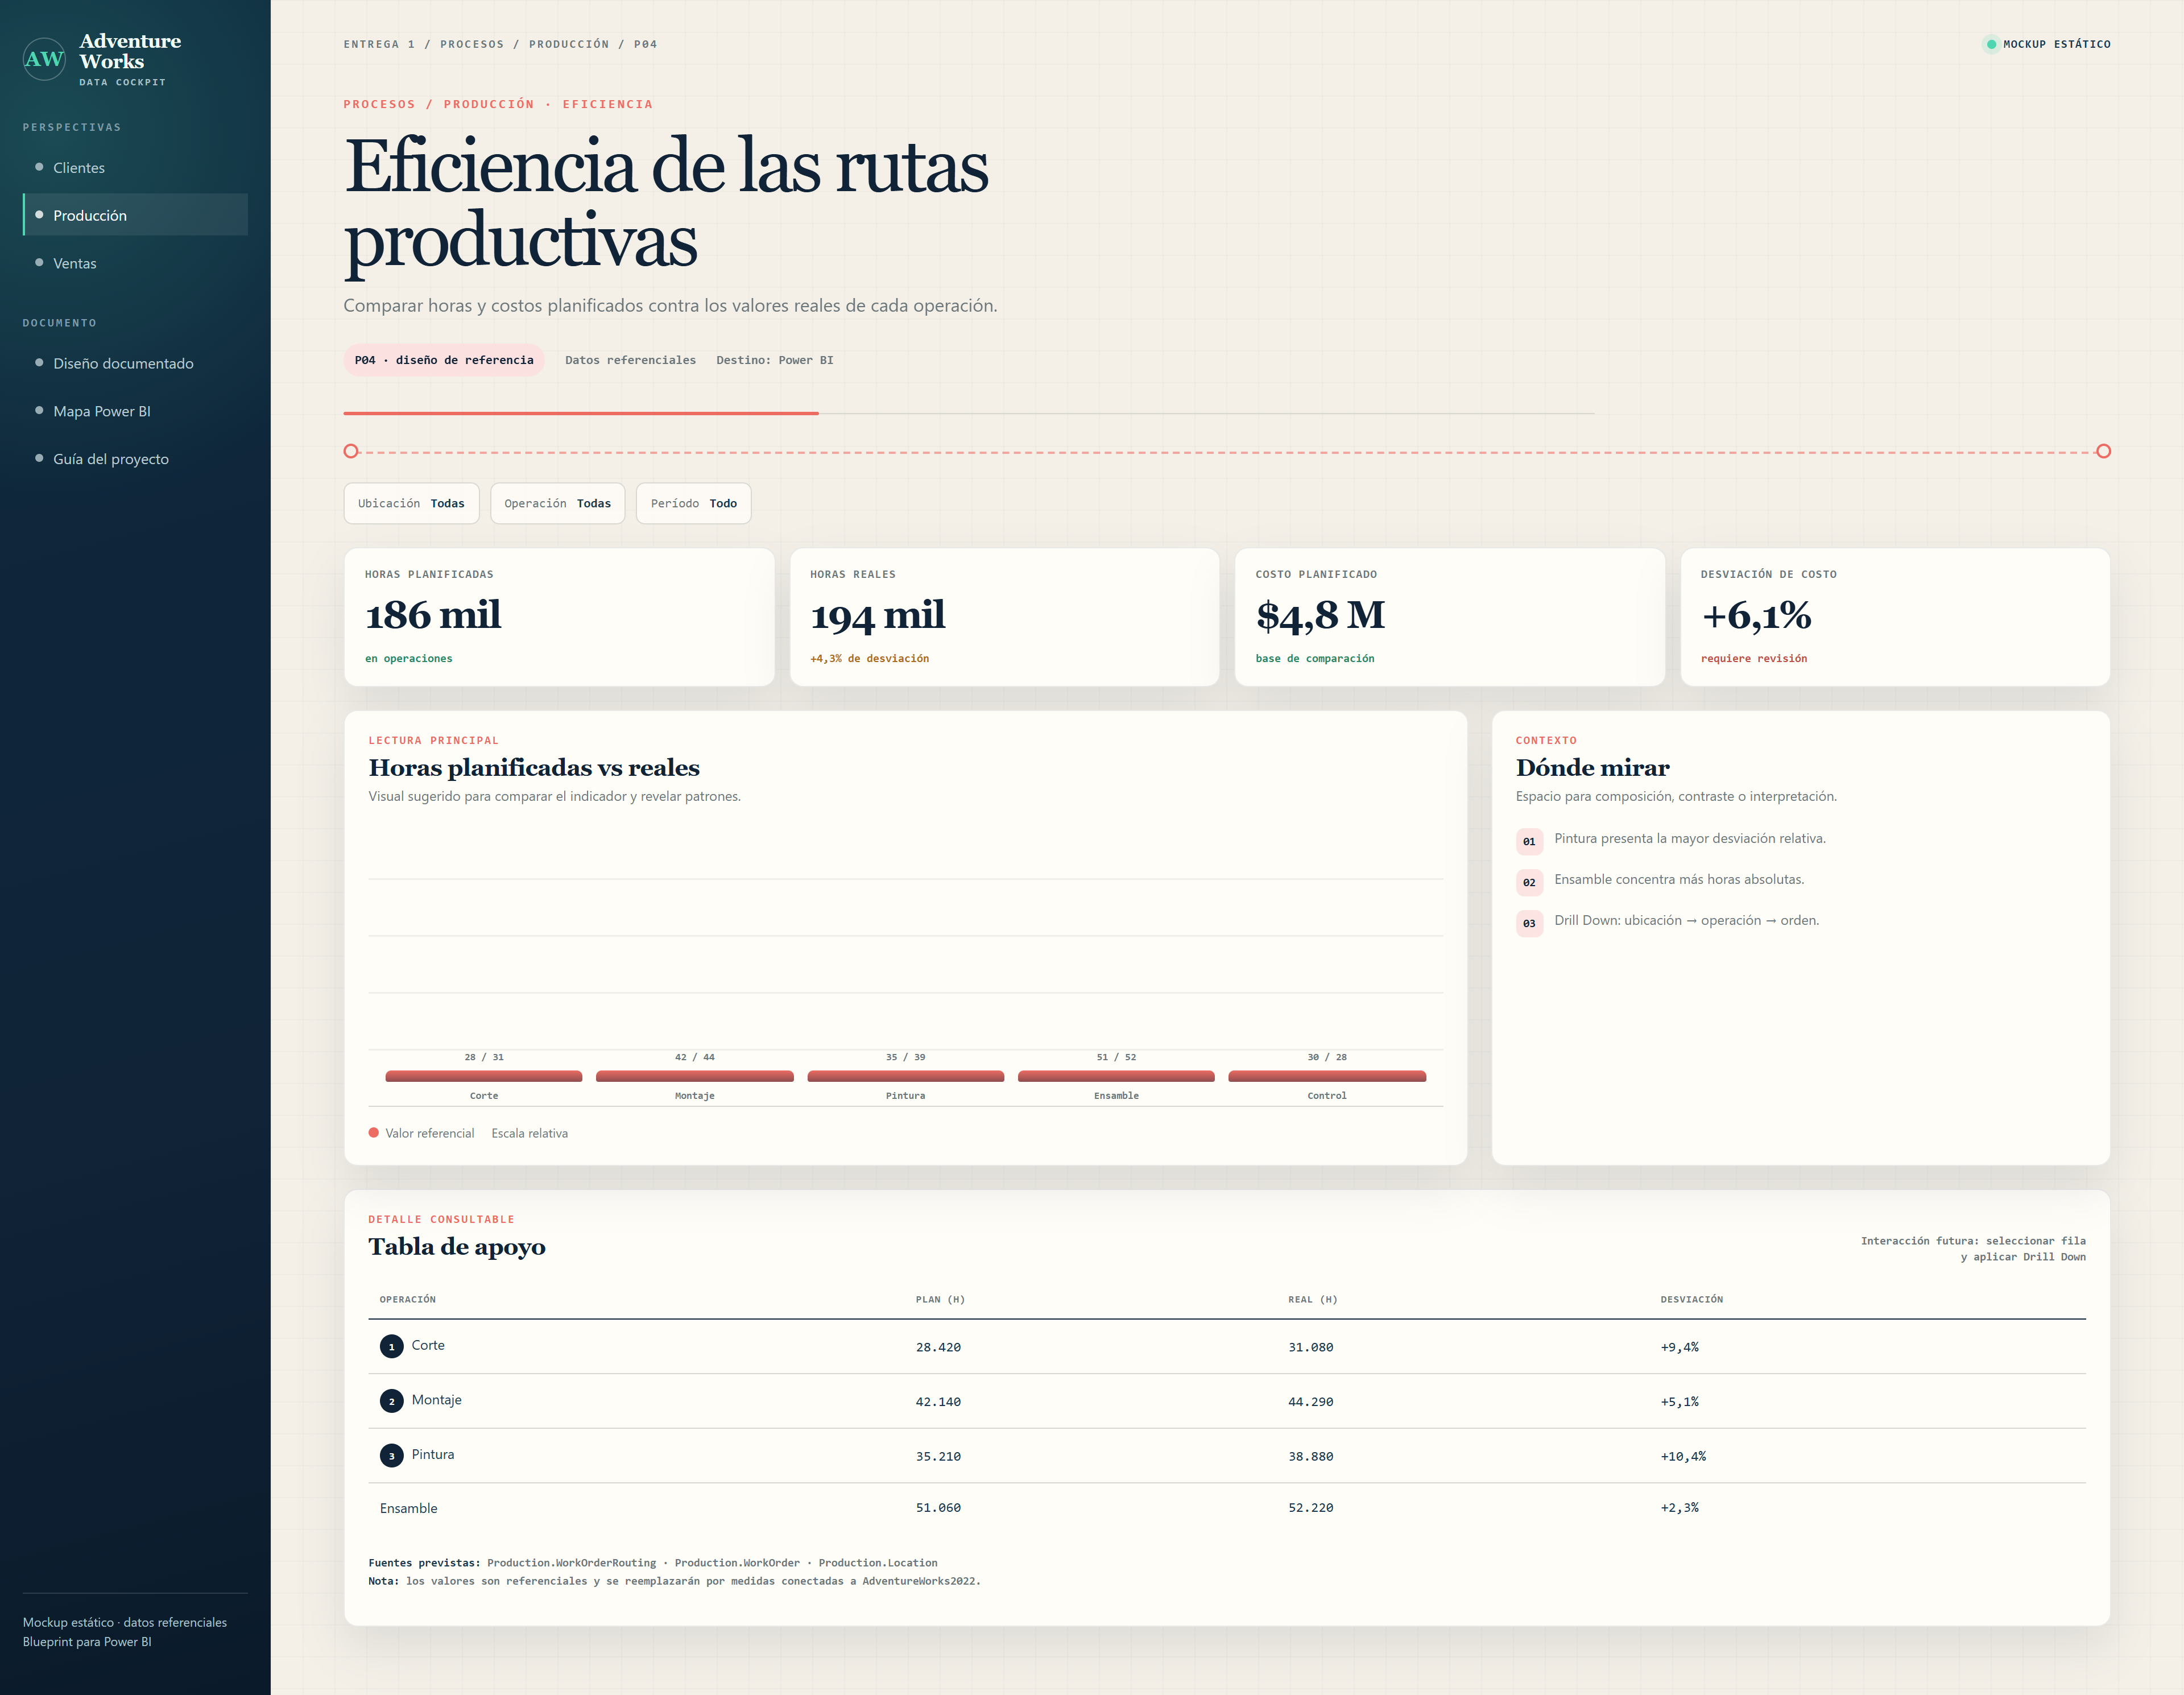
\includegraphics[width=0.84\textwidth]{mockup_produccion_04-eficiencia-rutas.png}
        \caption{Reporte P4: Eficiencia de las rutas productivas.}
    \end{figure}
    
    \clearpage
    \item \textbf{P5. Abastecimiento y proveedores:} Controlar compras operativas. Medirá órdenes de compra, monto y proveedores activos.
    \nopagebreak
    \begin{figure}[H]
        \centering
        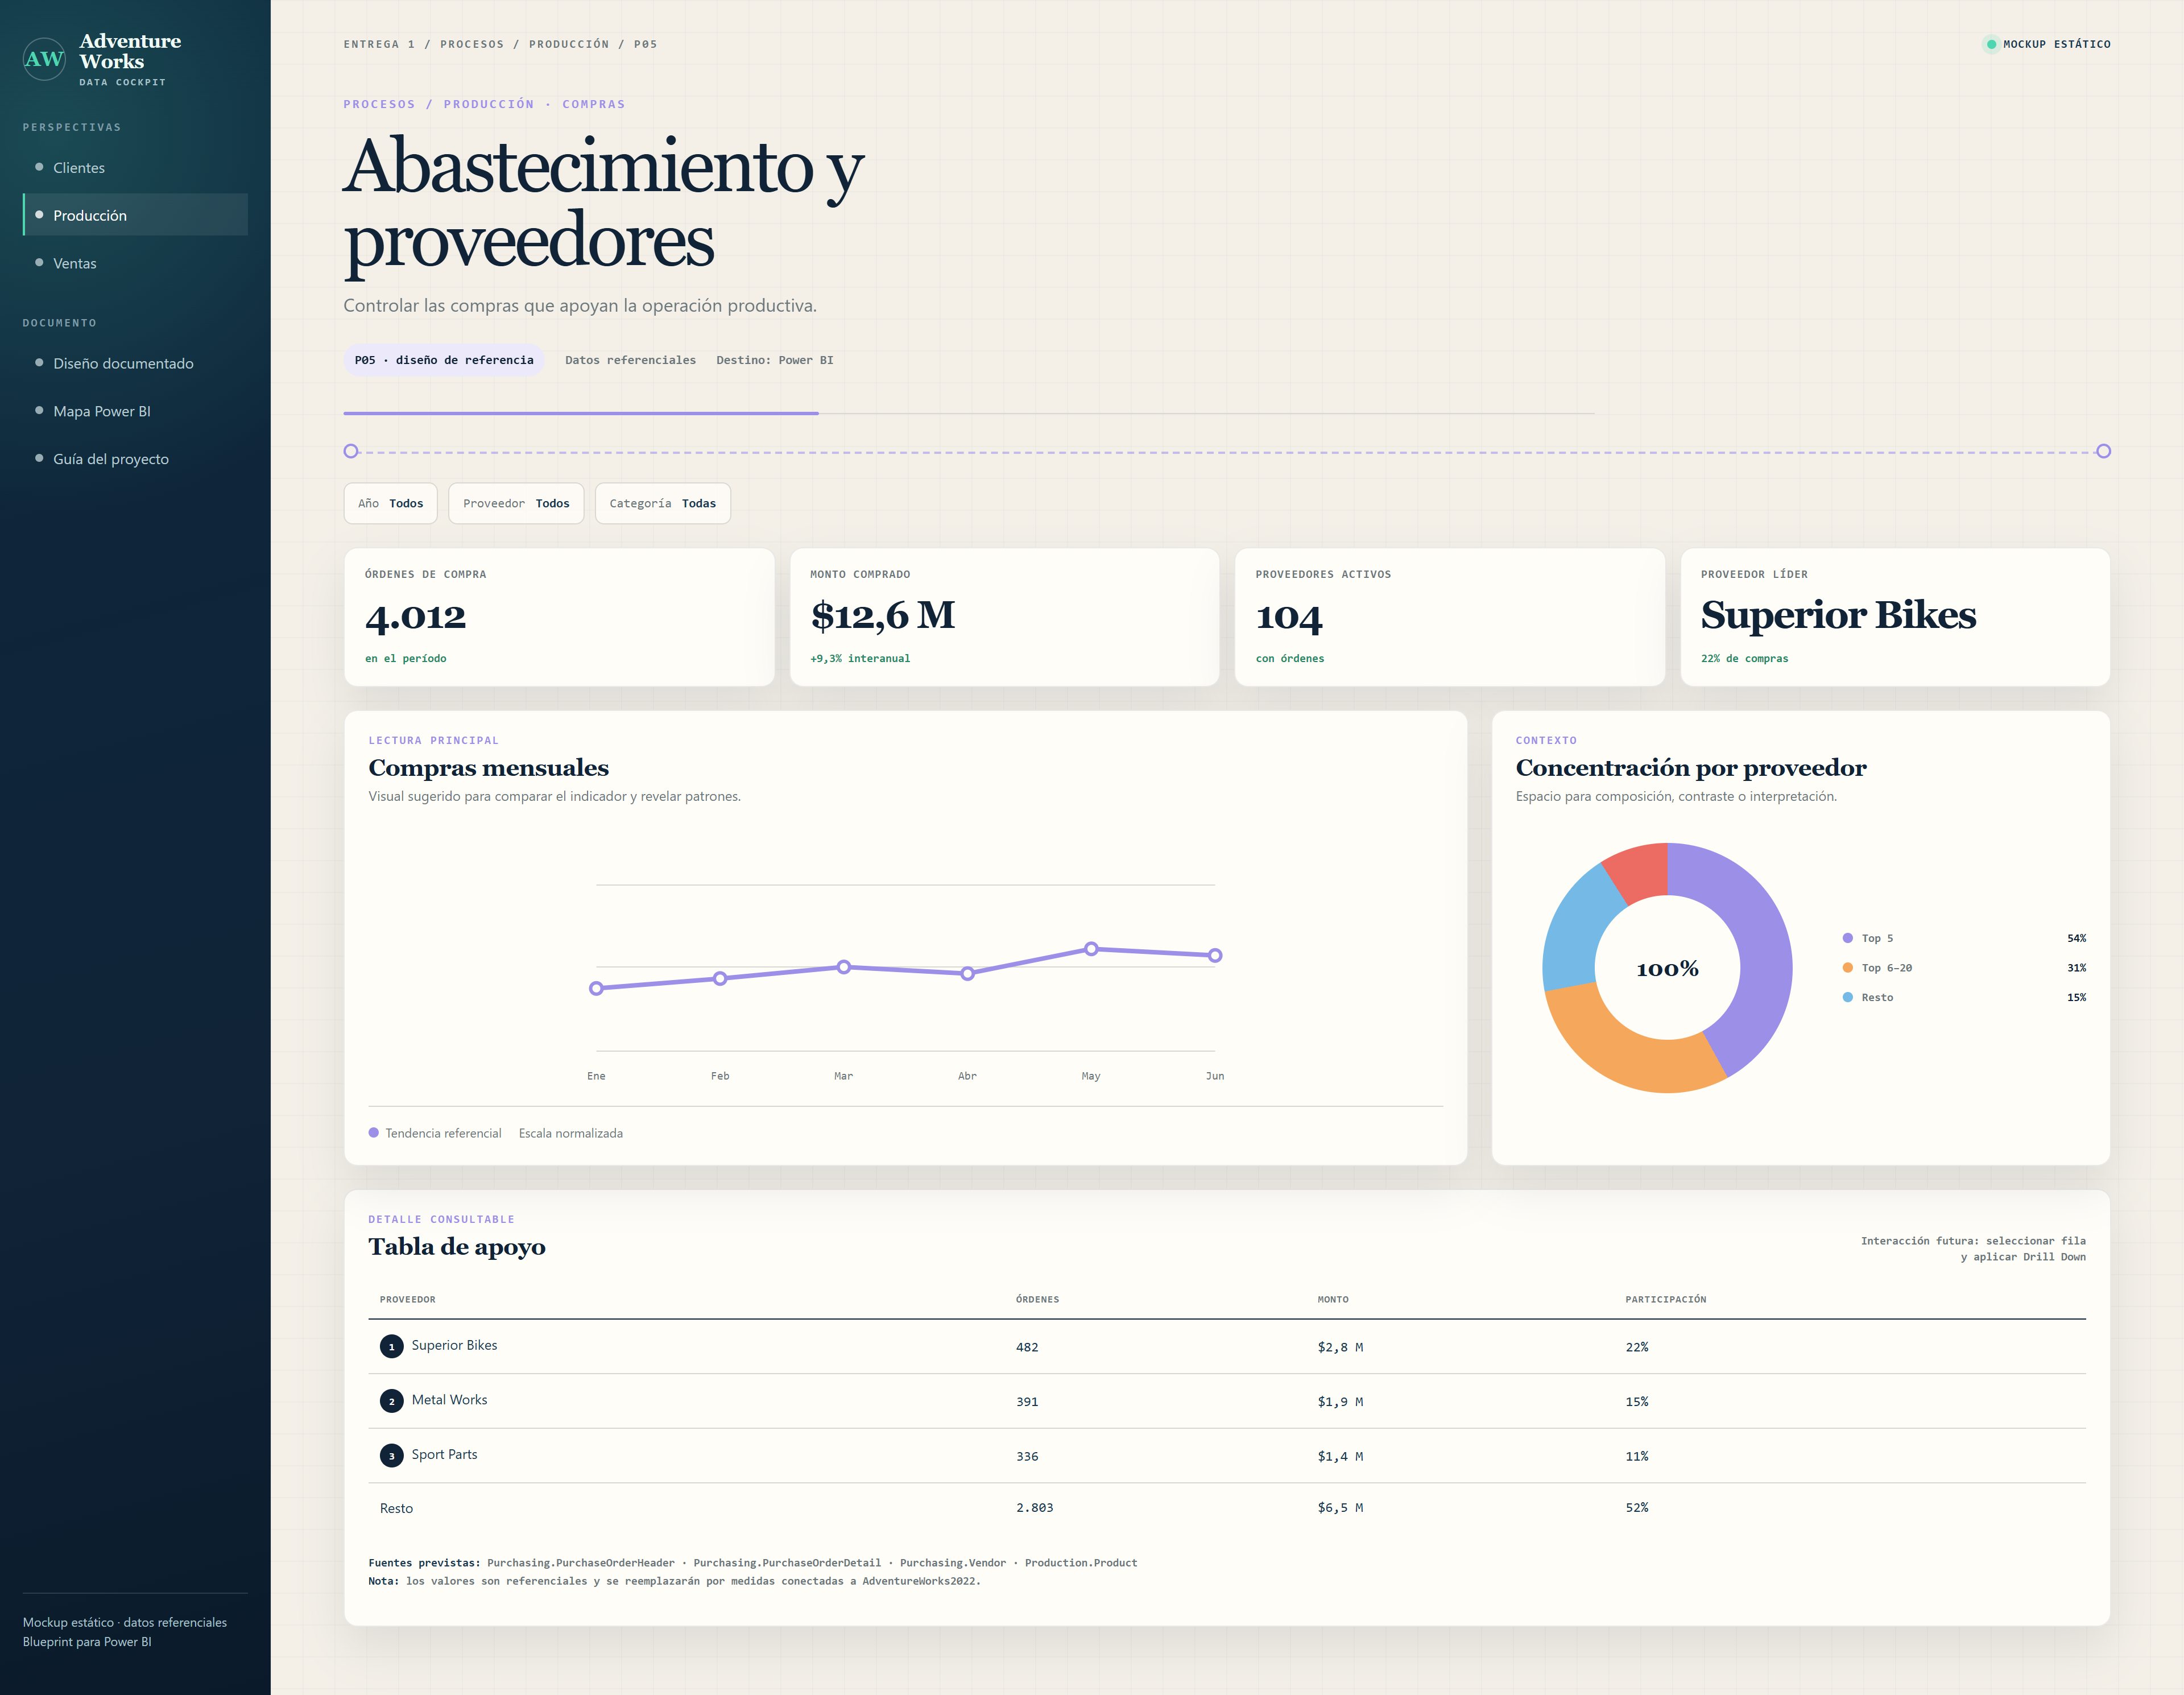
\includegraphics[width=0.84\textwidth]{mockup_produccion_05-abastecimiento-proveedores.png}
        \caption{Reporte P5: Abastecimiento y proveedores.}
    \end{figure}
\end{enumerate}

\clearpage
%-----------------------------------------------------------------------

\subsection{Perspectiva de Ventas}
Se proponen los siguientes 5 reportes:
\begin{enumerate}
    \item \textbf{V1. Resumen ejecutivo de ventas:} Vista general del desempeño. Medirá ventas totales, órdenes y ticket promedio.
    \nopagebreak
    \begin{figure}[H]
        \centering
        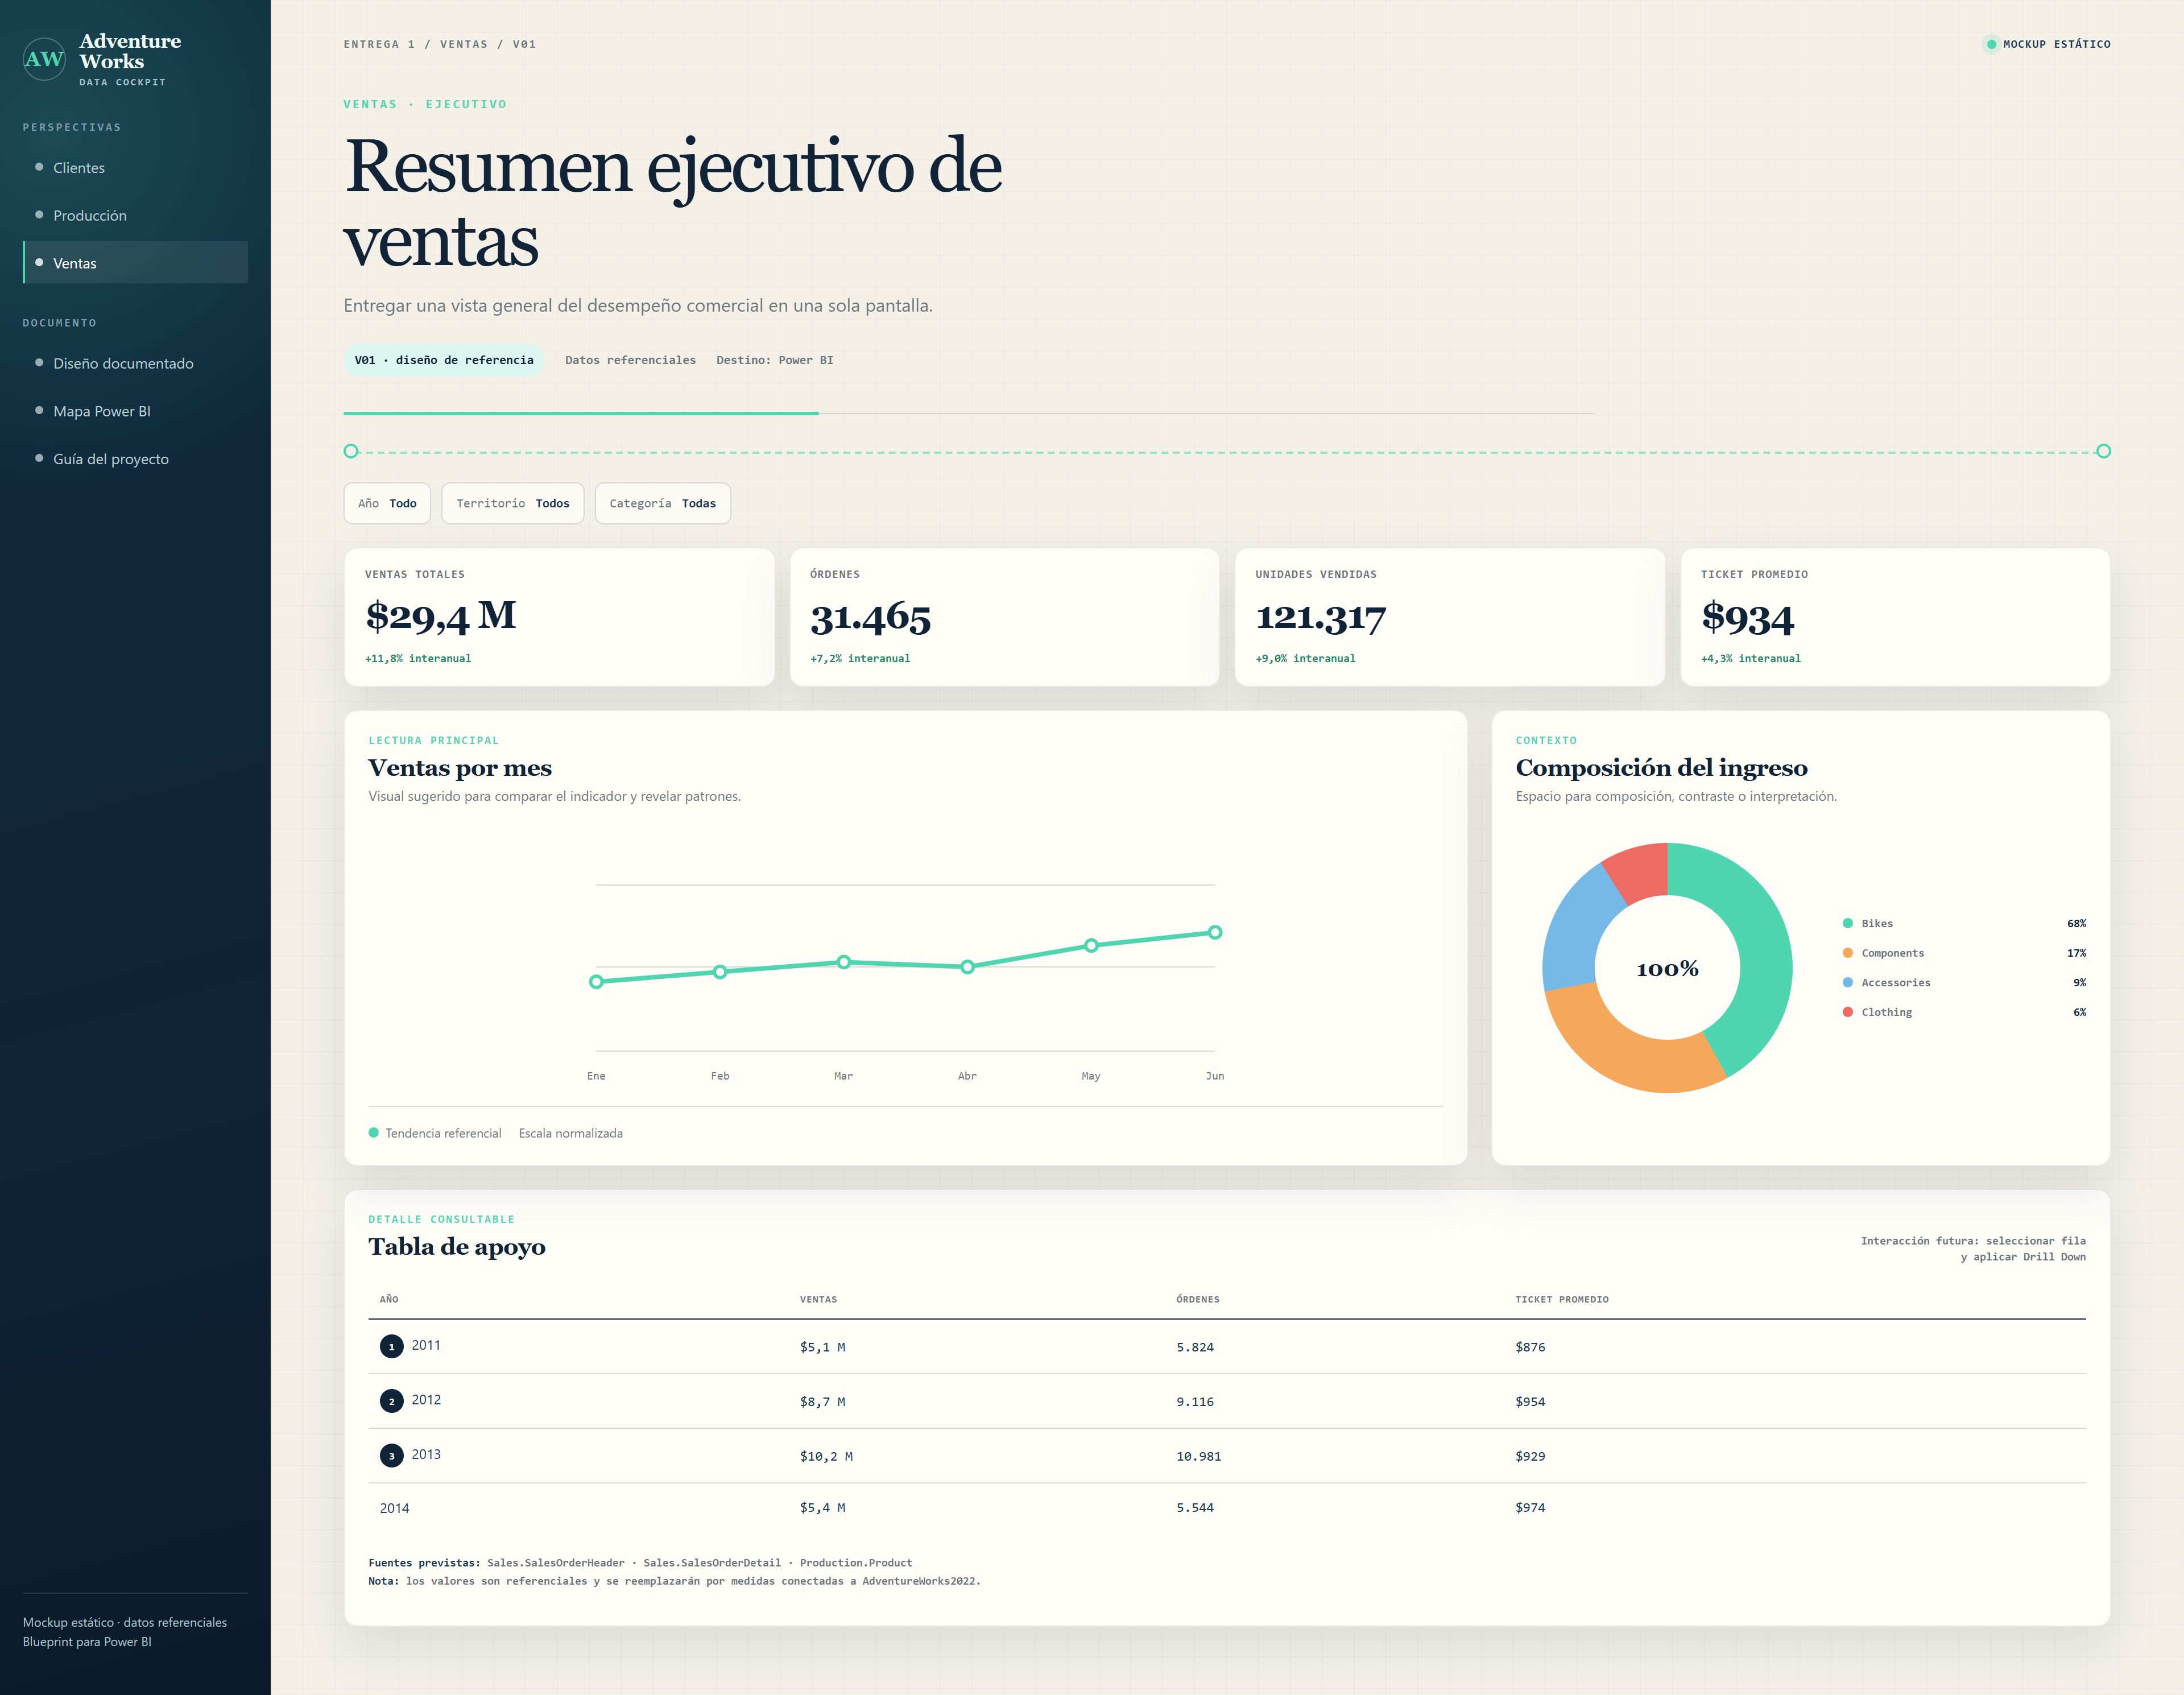
\includegraphics[width=0.82\textwidth]{mockup_ventas_01-resumen-ventas.png}
        \caption{Reporte V1: Resumen ejecutivo de ventas.}
    \end{figure}
    
    \clearpage
    \item \textbf{V2. Ventas por territorio:} Comparar el rendimiento regional. Medirá ventas, órdenes y variación por territorio.
    \nopagebreak
    \begin{figure}[H]
        \centering
        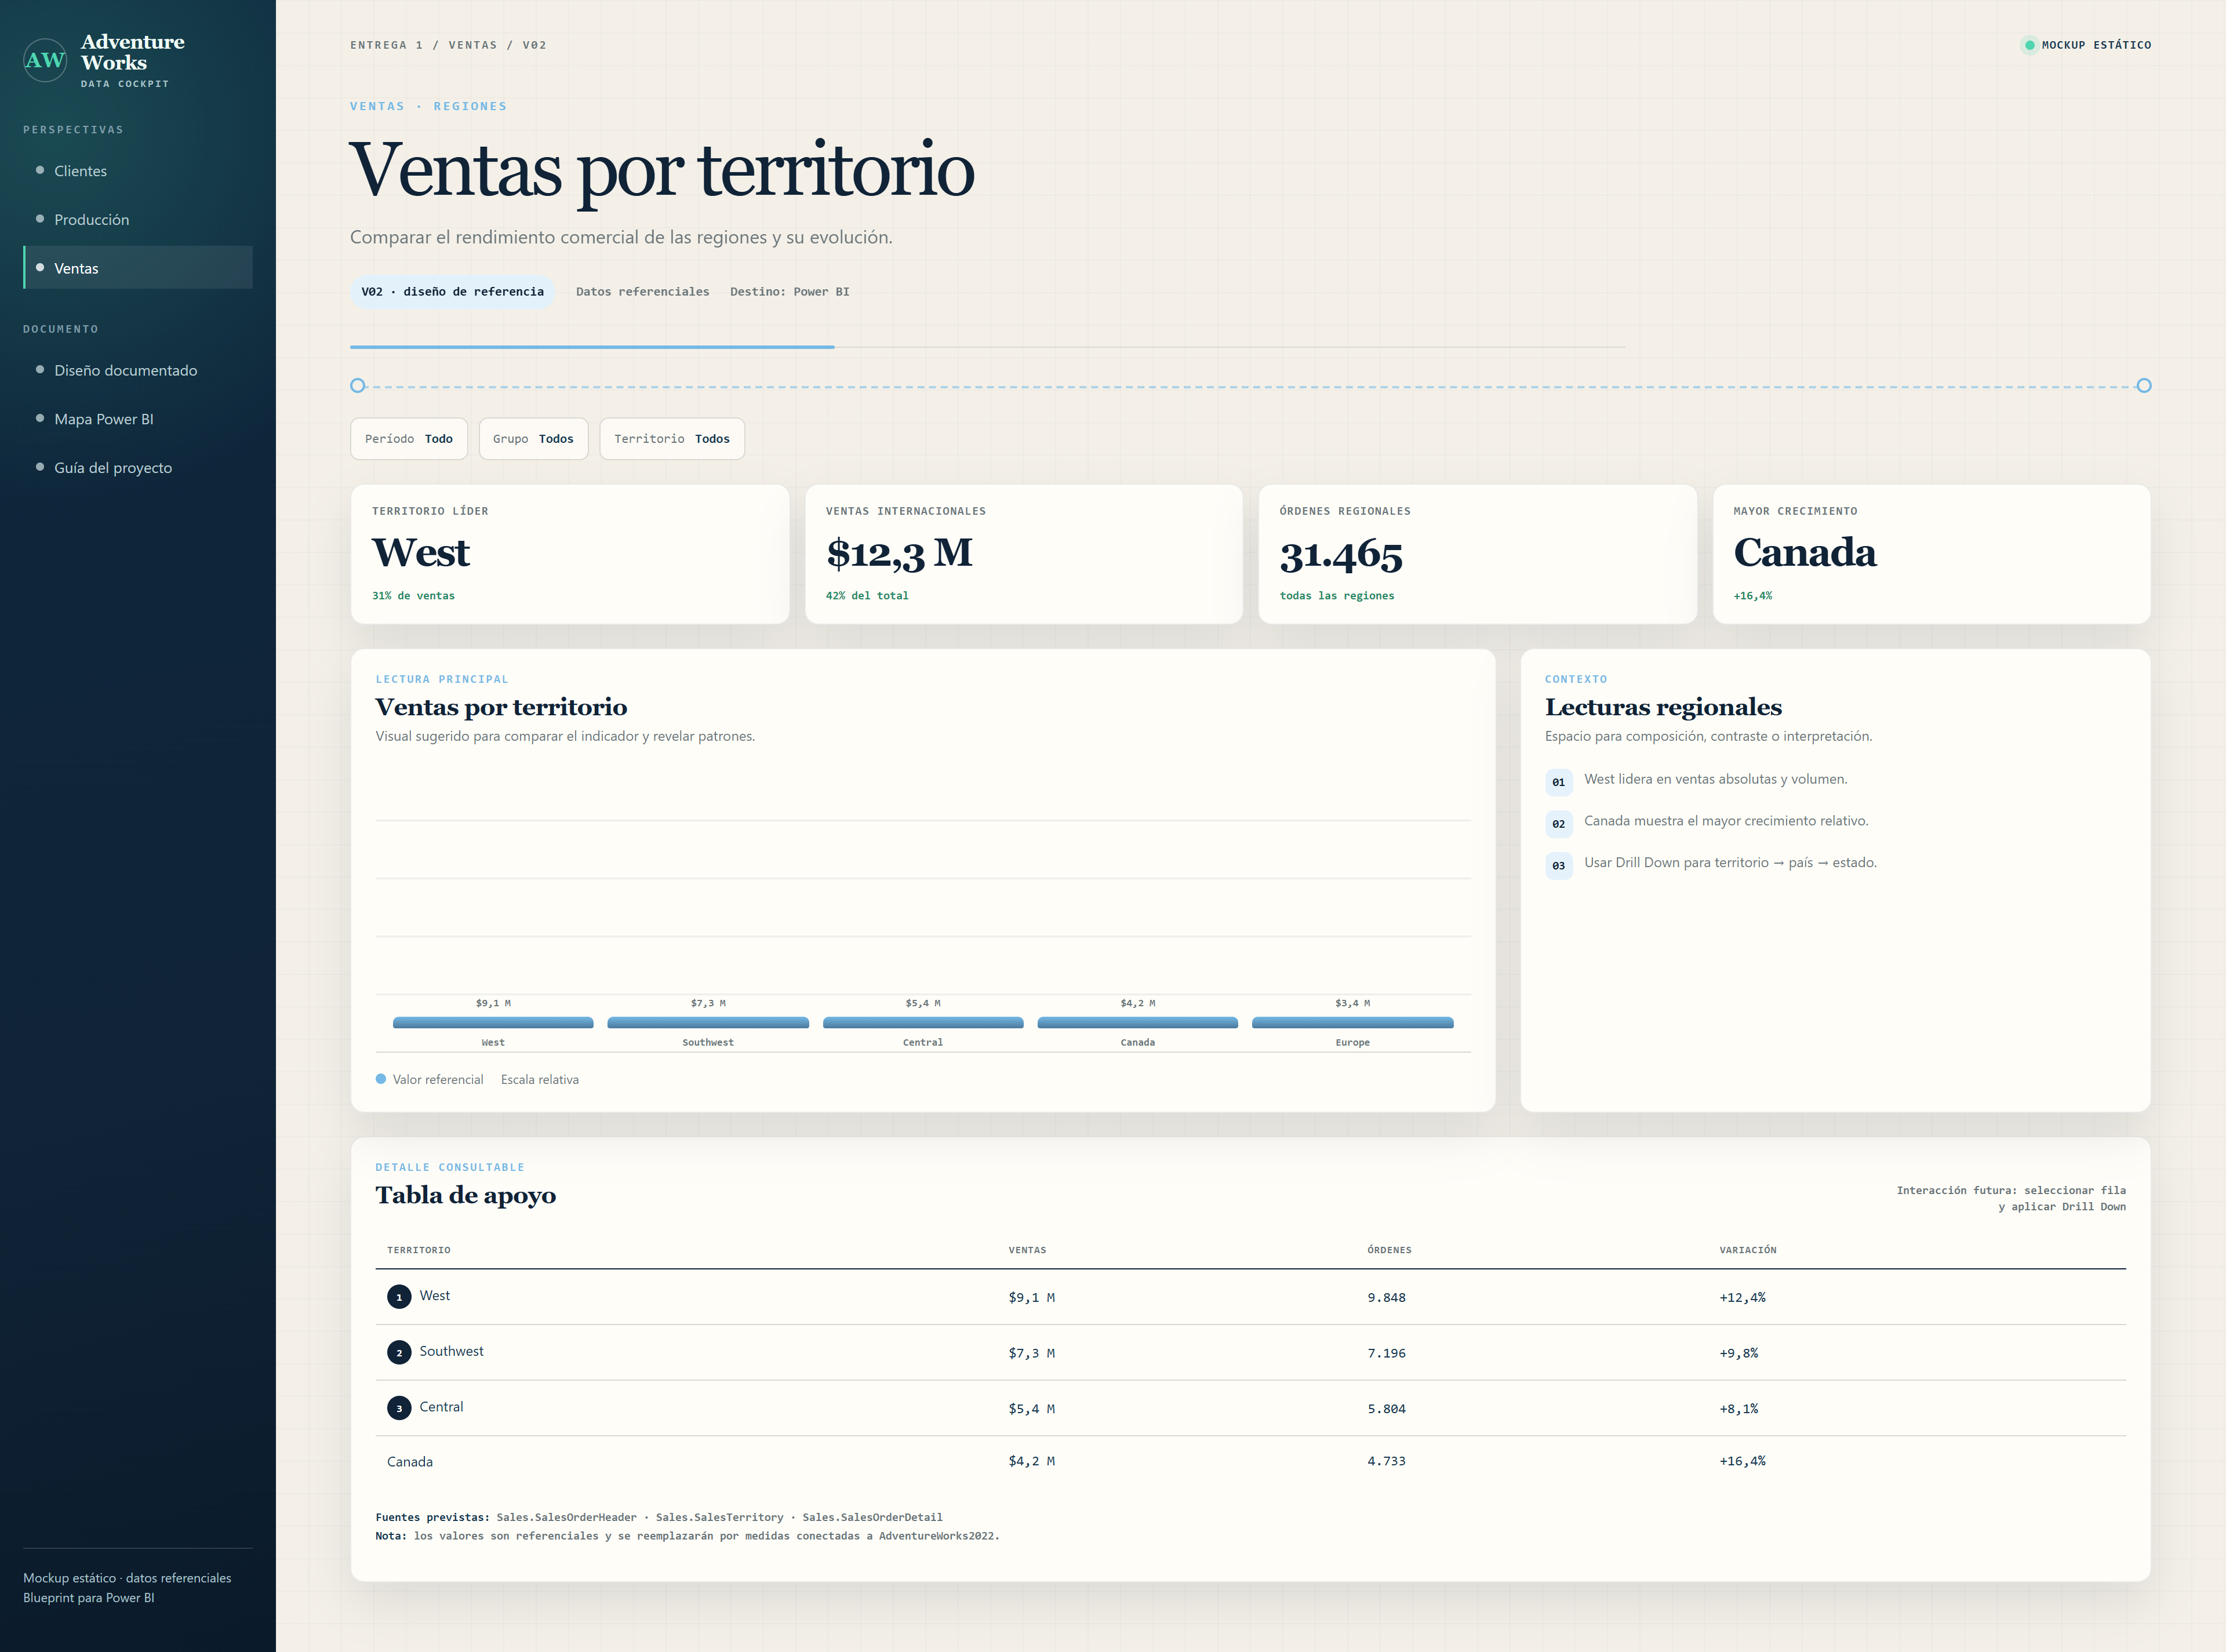
\includegraphics[width=0.84\textwidth]{mockup_ventas_02-ventas-territorio.png}
        \caption{Reporte V2: Ventas por territorio.}
    \end{figure}
    
    \clearpage
    \item \textbf{V3. Ventas por producto y categoría:} Identificar productos importantes. Medirá ventas, unidades y participación porcentual.
    \nopagebreak
    \begin{figure}[H]
        \centering
        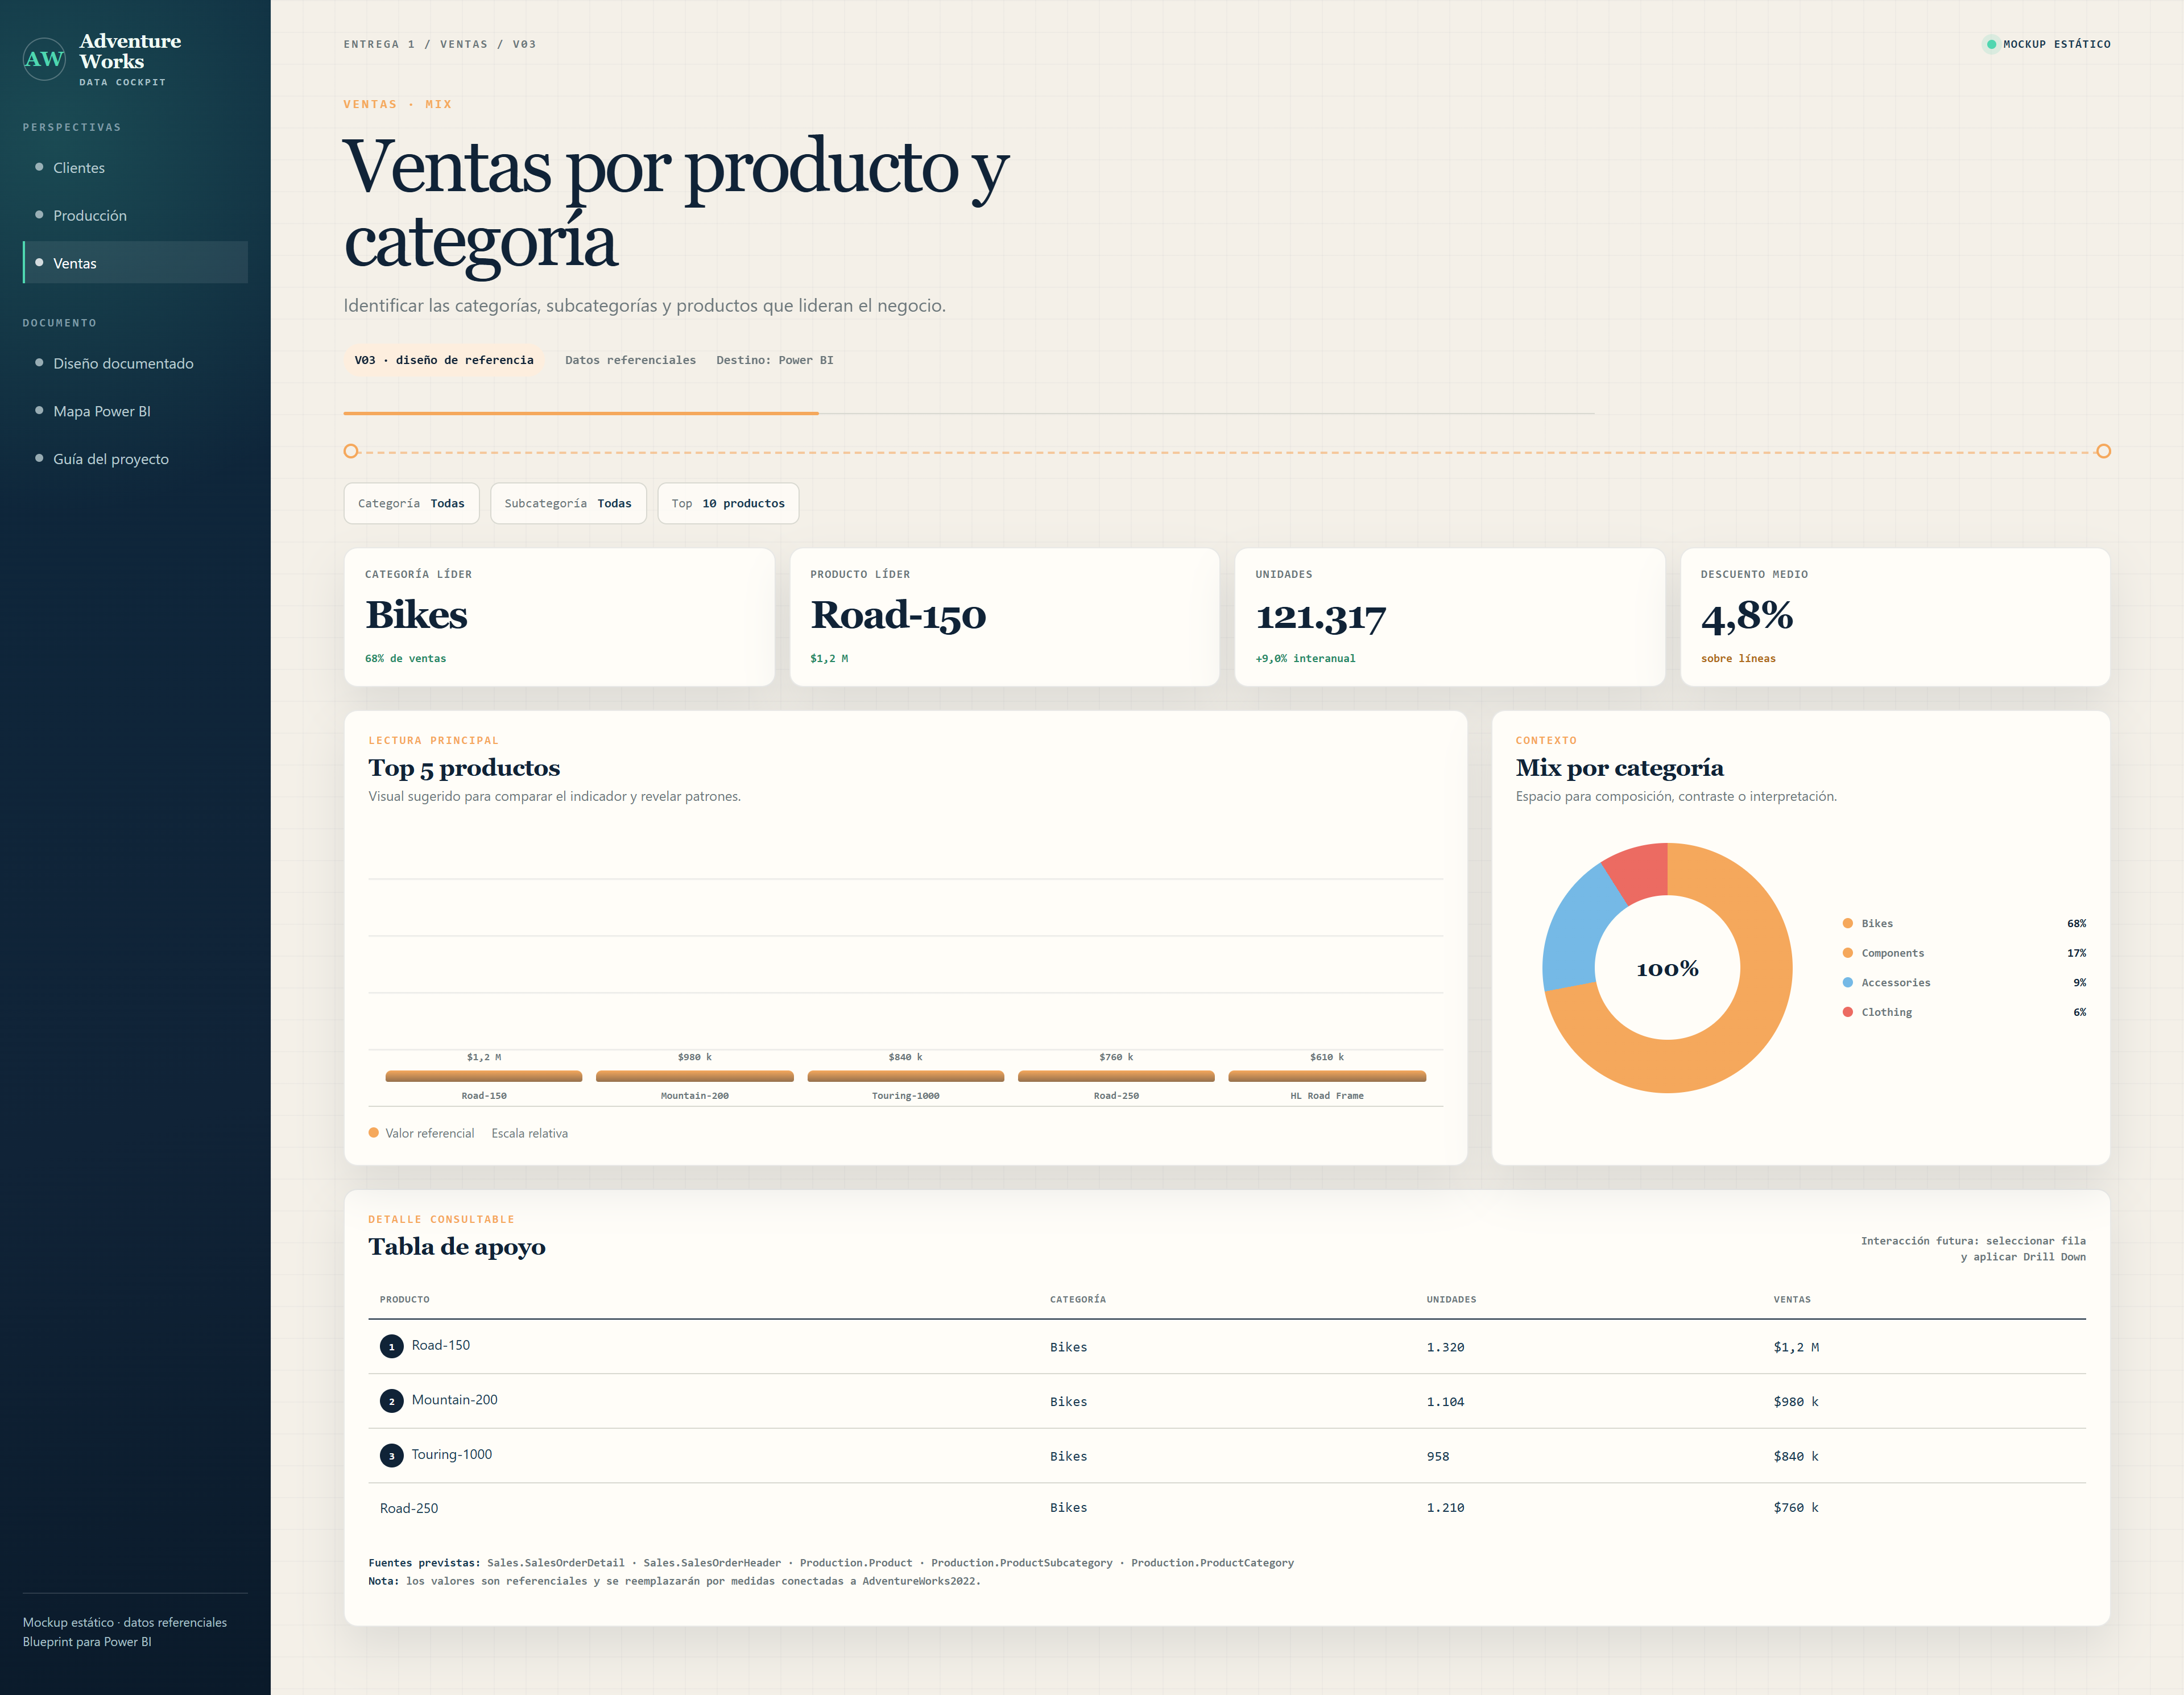
\includegraphics[width=0.84\textwidth]{mockup_ventas_03-ventas-producto.png}
        \caption{Reporte V3: Ventas por producto y categoría.}
    \end{figure}
    
    \clearpage
    \item \textbf{V4. Ventas online vs. distribuidor:} Comparar canales. Medirá porcentaje online y ticket promedio por canal.
    \nopagebreak
    \begin{figure}[H]
        \centering
        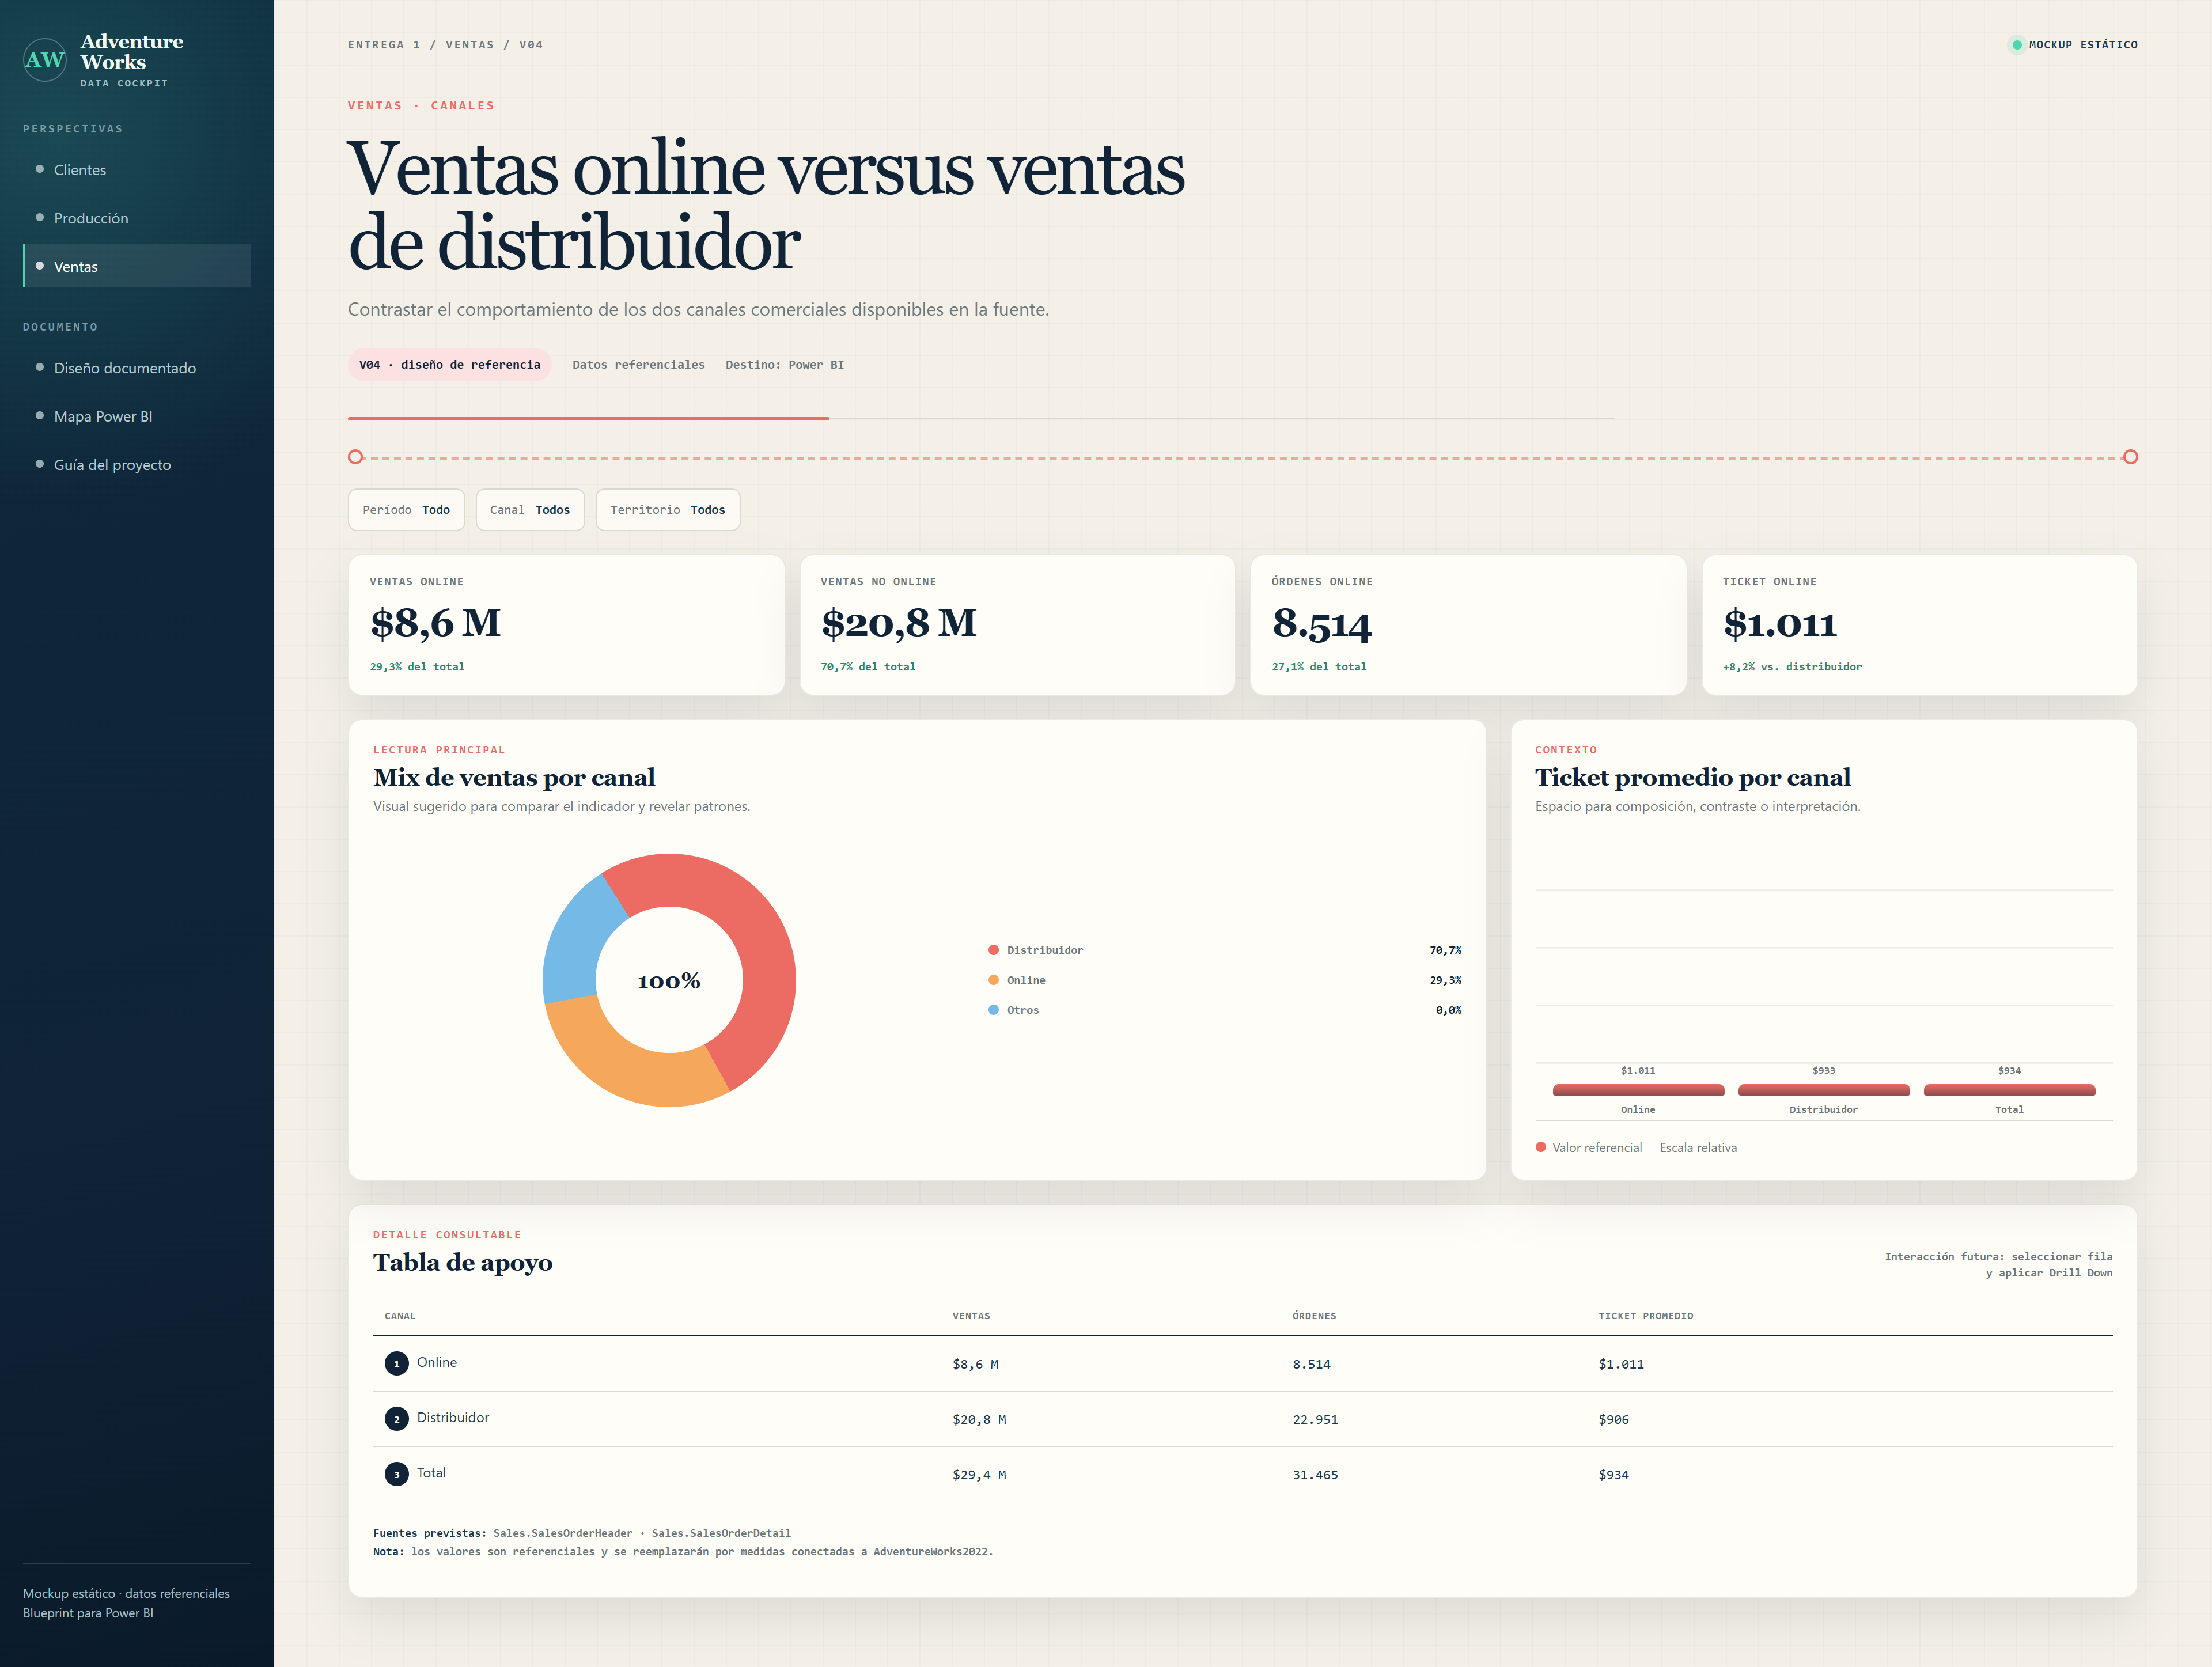
\includegraphics[width=0.84\textwidth]{mockup_ventas_04-ventas-canal.png}
        \caption{Reporte V4: Ventas online vs distribuidor.}
    \end{figure}
    
    \clearpage
    \item \textbf{V5. Desempeño de vendedores:} Analizar la contribución por vendedor. Medirá ventas, órdenes y comparación con año anterior.
    \nopagebreak
    \begin{figure}[H]
        \centering
        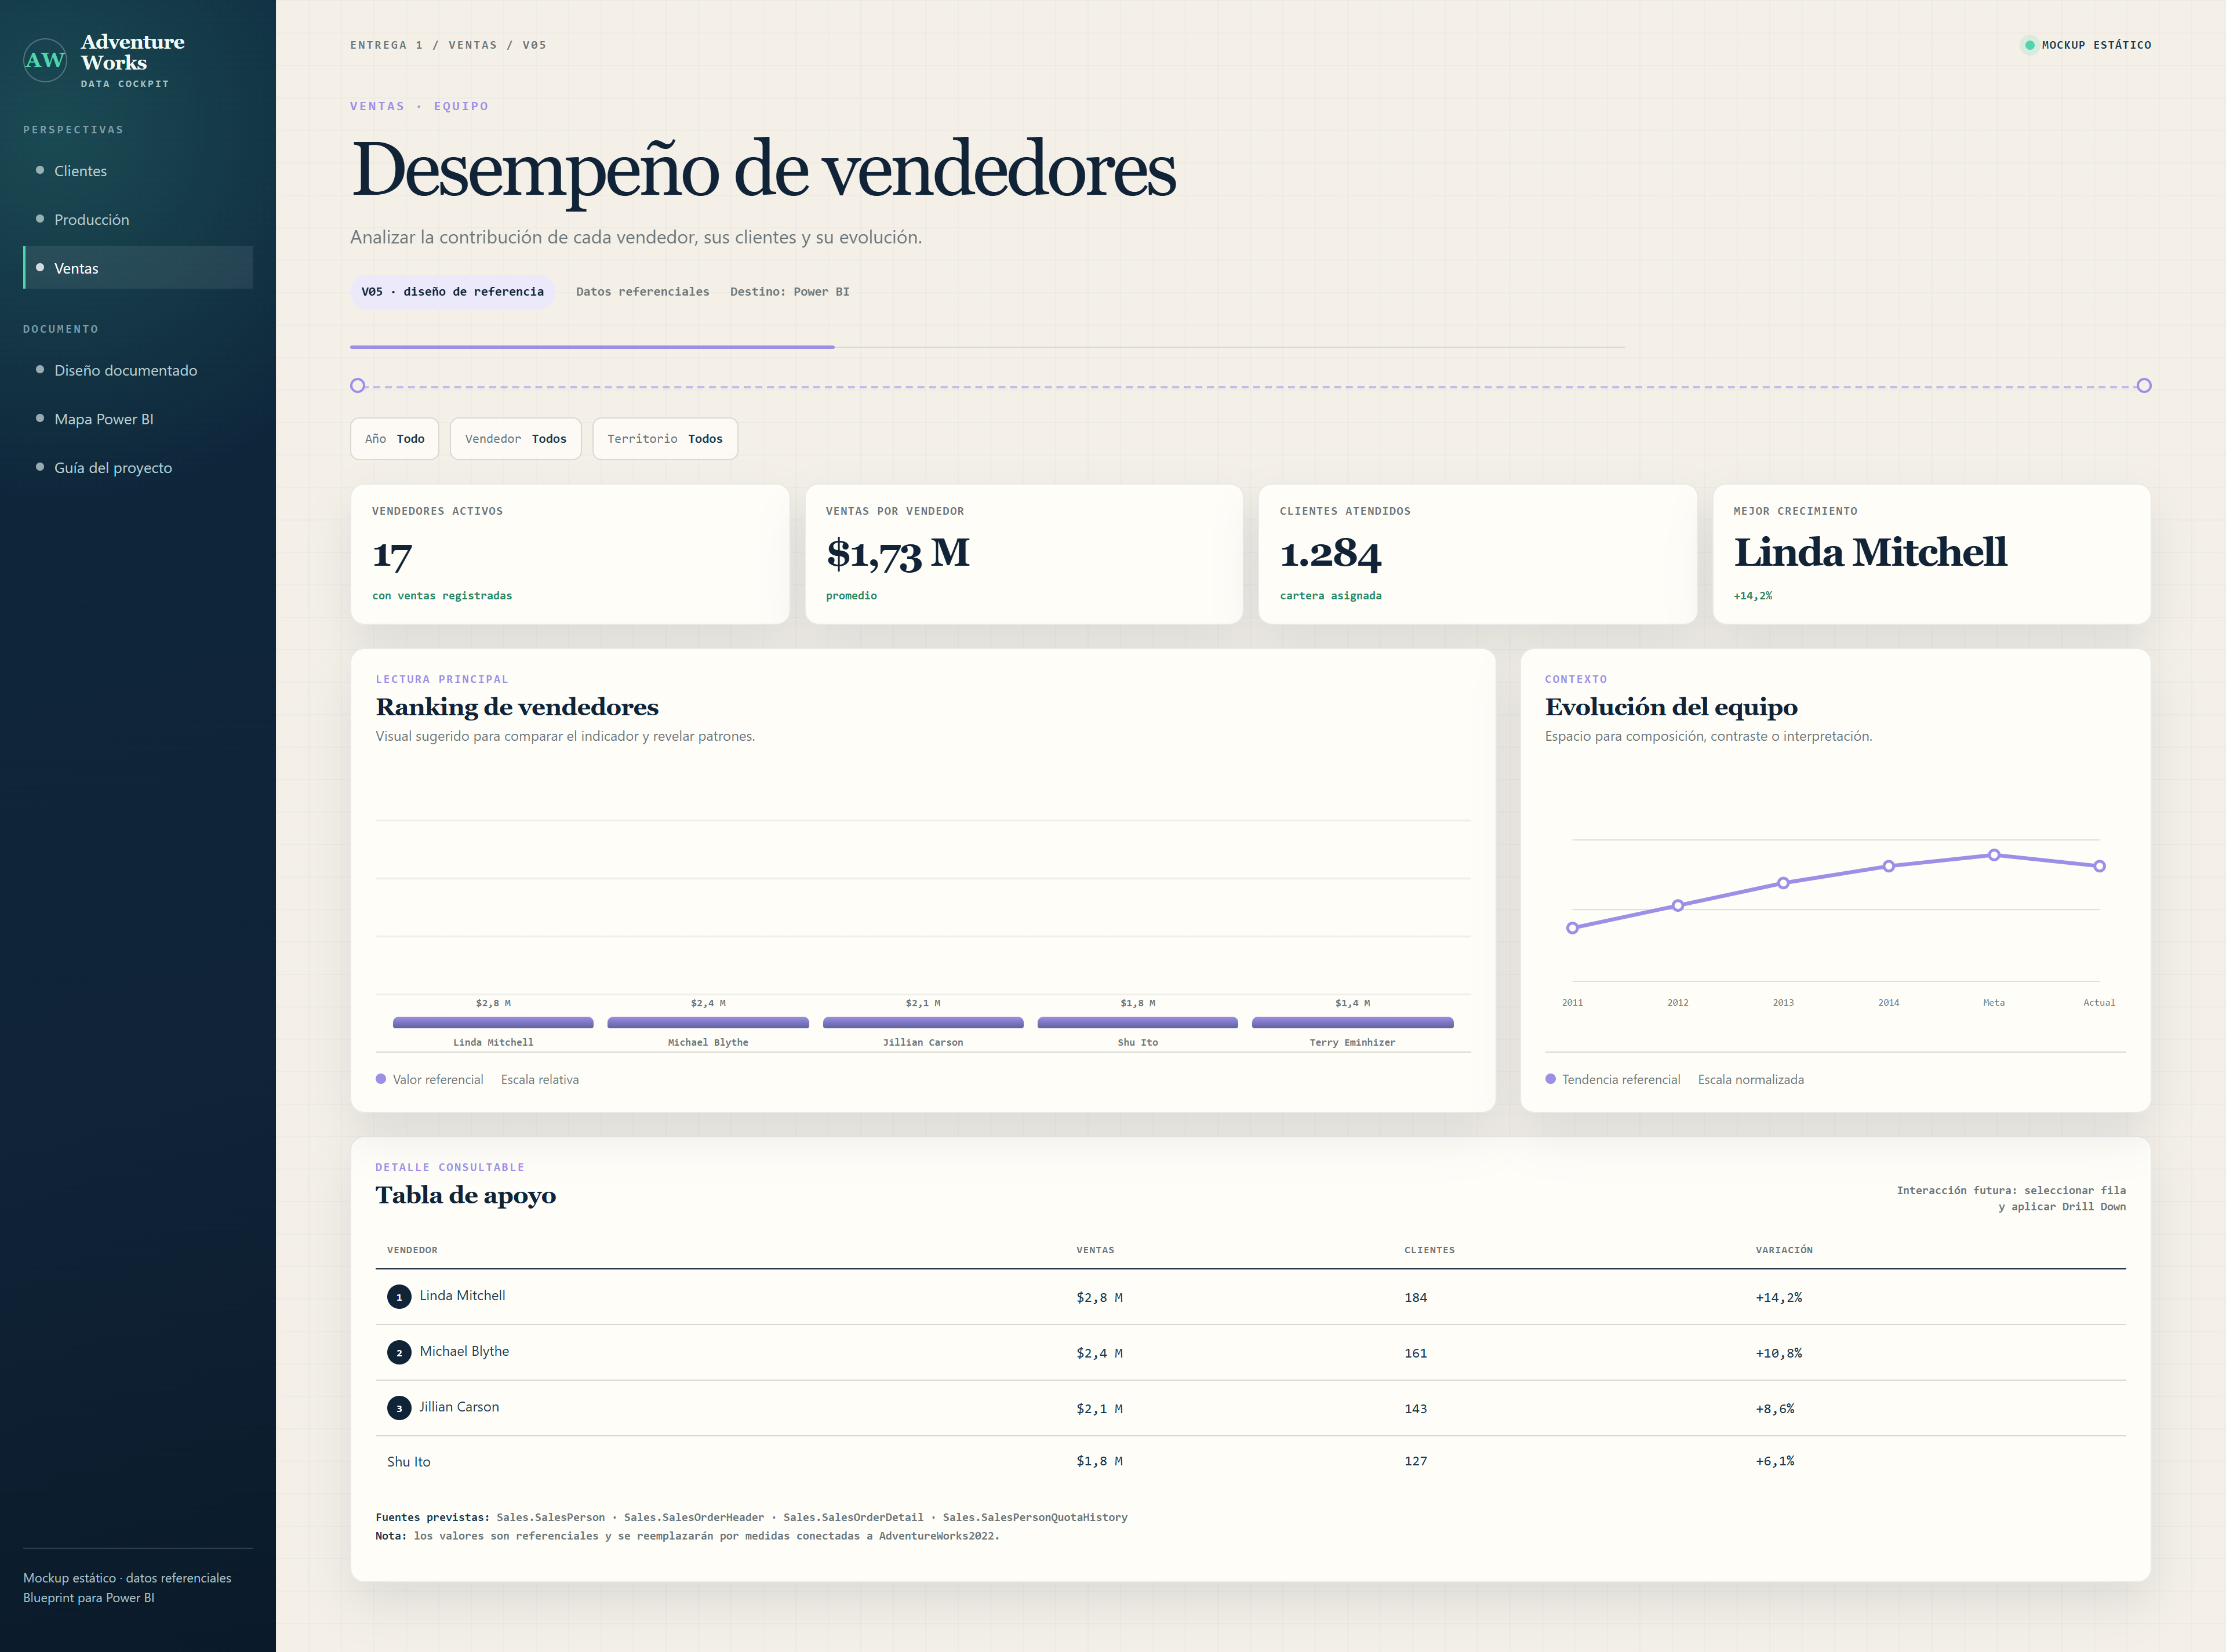
\includegraphics[width=0.84\textwidth]{mockup_ventas_05-desempeno-vendedores.png}
        \caption{Reporte V5: Desempeño de vendedores.}
    \end{figure}
\end{enumerate}

\vspace{0.4cm}
\textbf{Nota sobre Drill Down:} Tal como se indica en las bonificaciones del proyecto, se implementará navegación Drill Down en estos reportes, permitiendo bajar de Categoría a Producto, o de Año a Mes.

%-----------------------------------------------------------------------

\clearpage
\section{Base de Datos Transaccional Implementada}
En esta sección se evidencia la correcta restauración e implementación de la base de datos \texttt{AdventureWorks2022} configurada como fuente de datos operativa para el proyecto.

\begin{figure}[H]
    \centering
    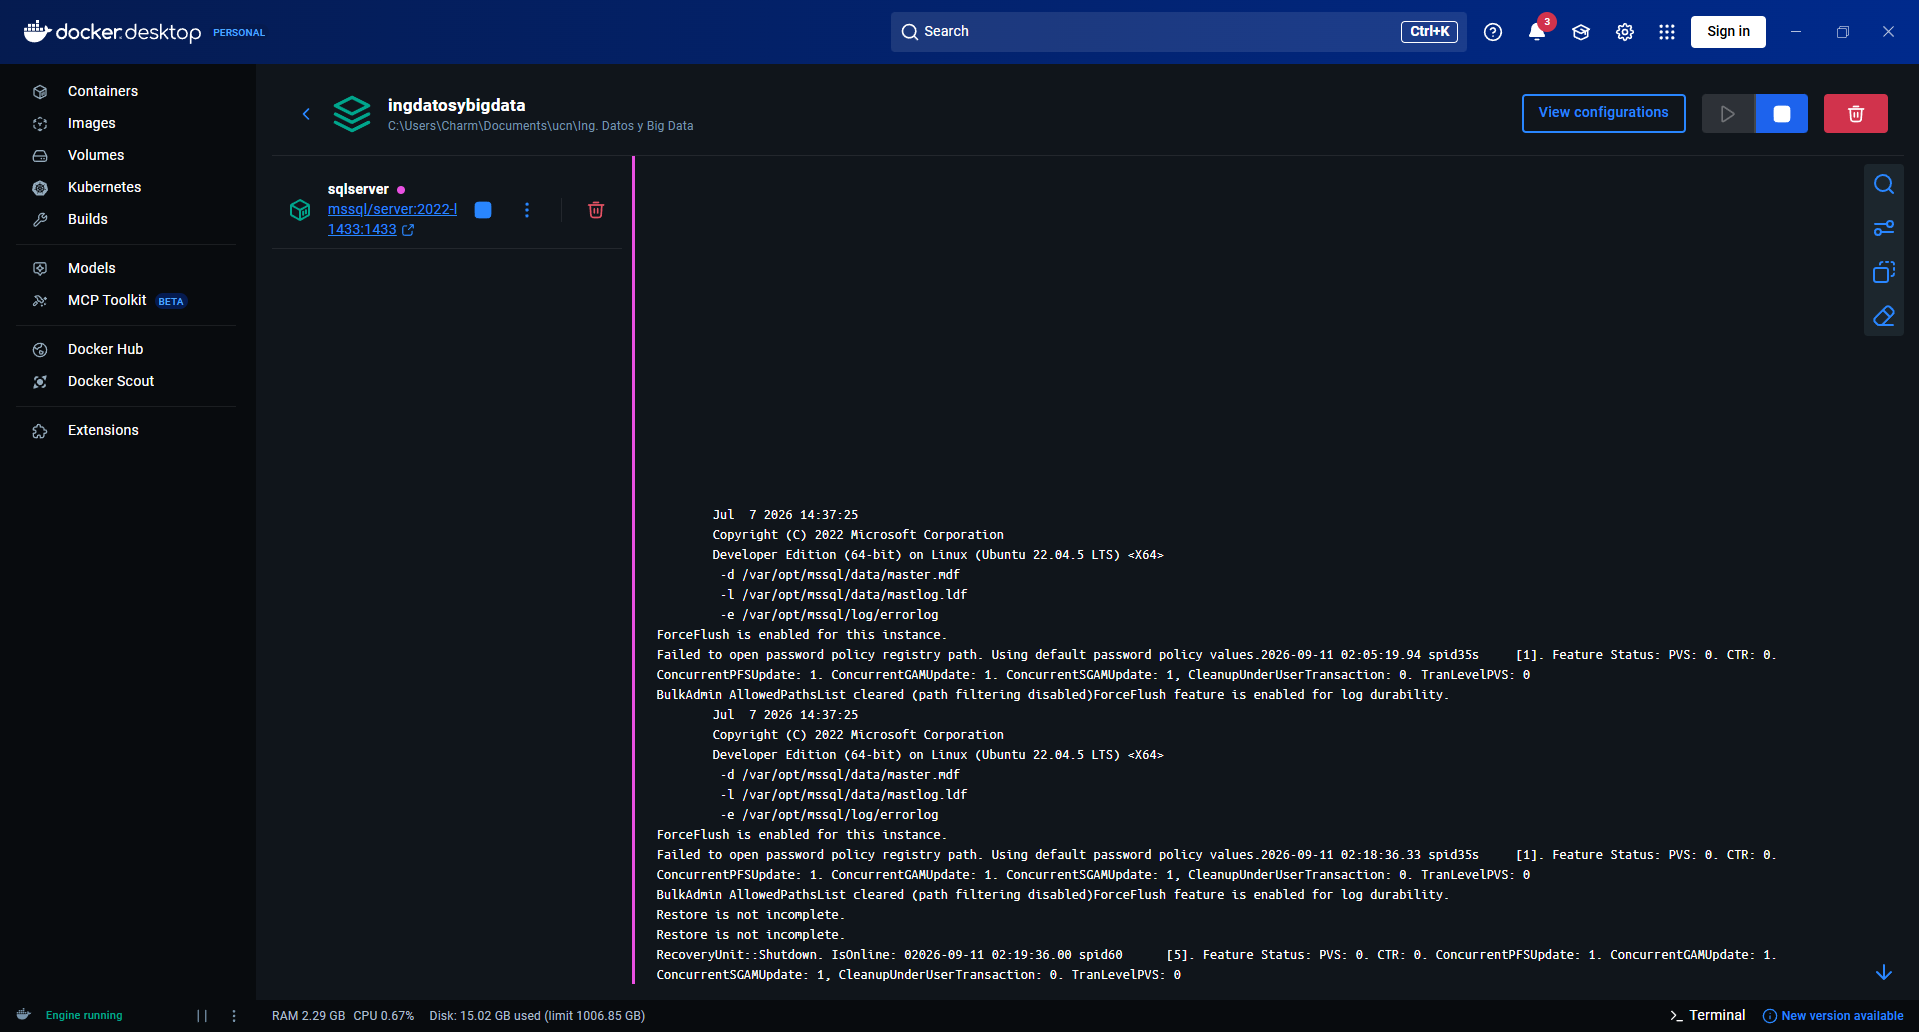
\includegraphics[width=0.76\textwidth]{evidencia_sql1.png}
    \caption{Vista del contenedor Docker ejecutando SQL Server.}
\end{figure}

\begin{figure}[H]
    \centering
    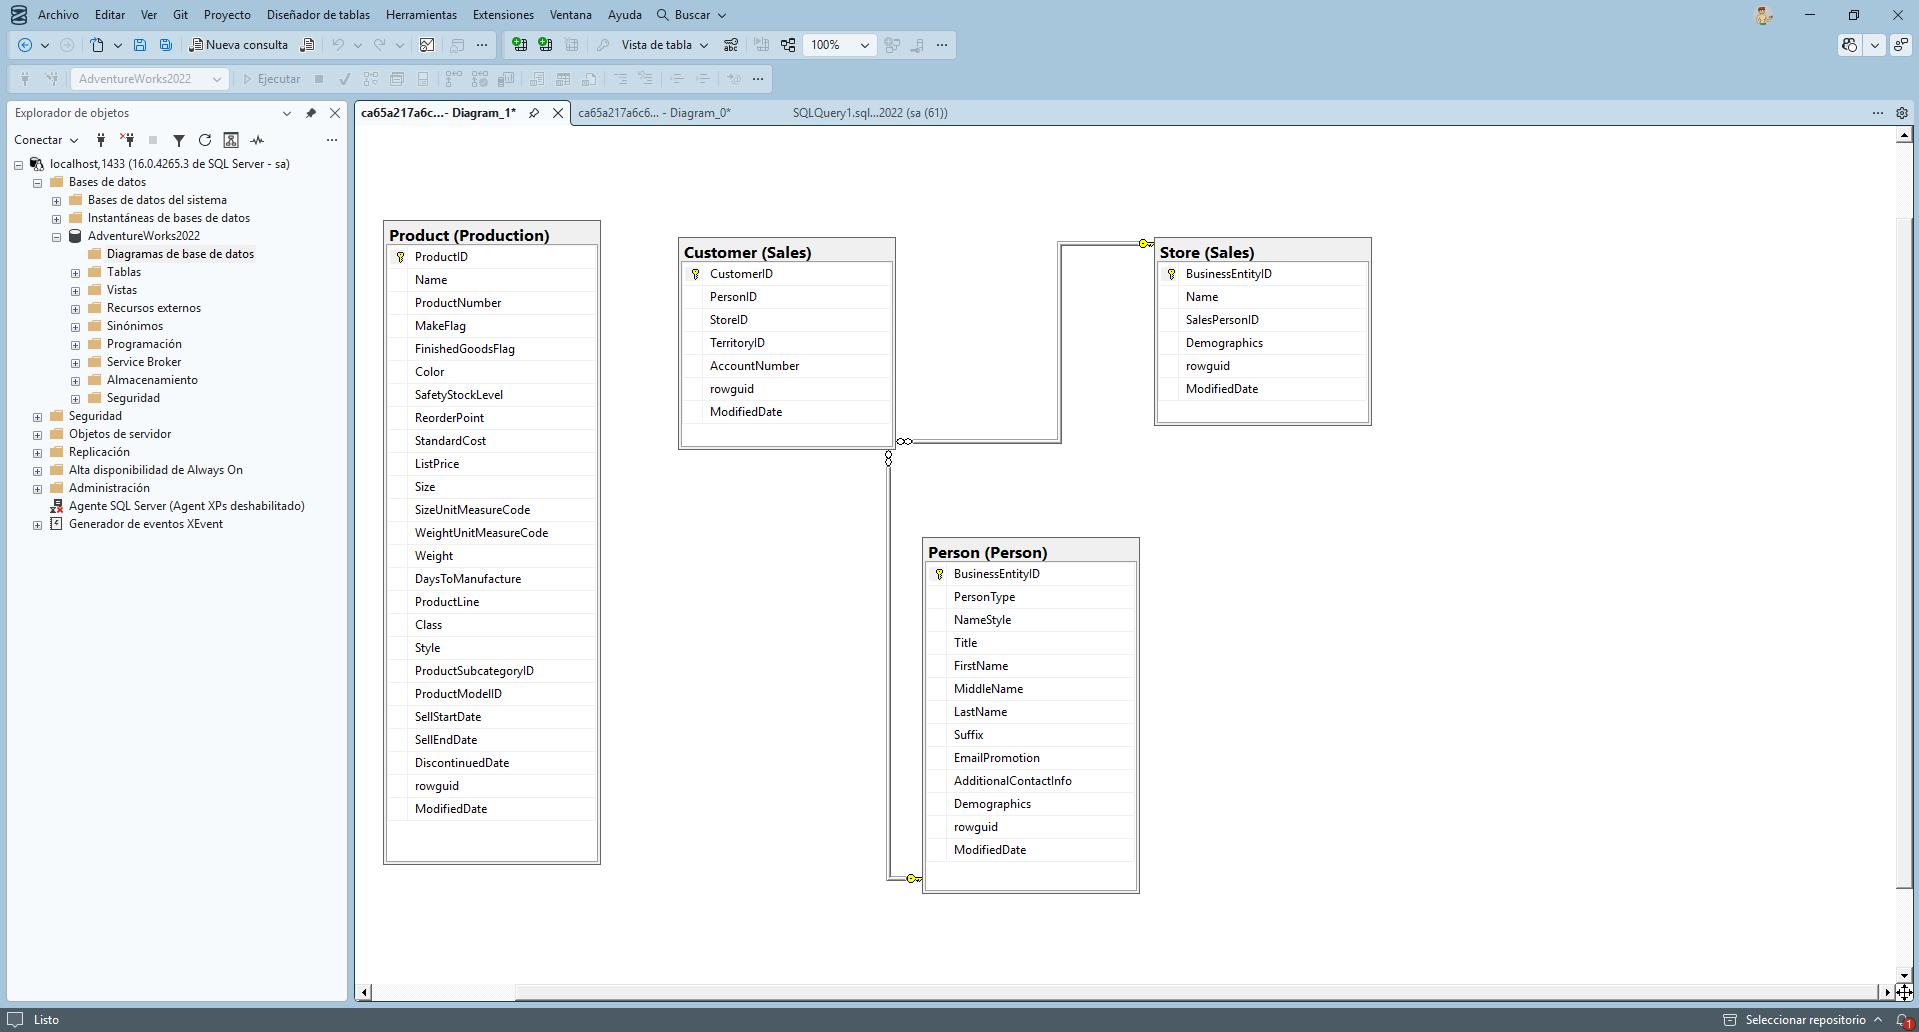
\includegraphics[width=0.76\textwidth]{evidencia_sql2.png}
    \caption{Base de datos AdventureWorks2022 visualizada en SQL Server Management Studio.}
\end{figure}

Como se observa en la evidencia, el motor se encuentra en funcionamiento. A modo de ejemplo, se generó un diagrama relacional con una pequeña muestra de las tablas que componen la base transaccional (\texttt{Product}, \texttt{Customer}, \texttt{Store} y \texttt{Person}). Esto confirma que la estructura importada reconoce correctamente los esquemas organizacionales (como \texttt{Production}, \texttt{Sales} y \texttt{Person}) y conserva sus relaciones originales, dejándola lista para la futura fase de extracción (ETL).

%-----------------------------------------------------------------------

\section{Conclusión}
En esta primera etapa se ha consolidado la base técnica y lógica del proyecto. Contar con la fuente transaccional operativa, junto con una arquitectura y diseños de reportes bien definidos, establece el punto de partida necesario para iniciar las tareas de integración (ETL) y modelado dimensional en las siguientes fases.

\end{document}